%!TeX program = xelatex
\documentclass[12pt,hyperref,a4paper,UTF8]{ctexart} 
\usepackage{booktabs}  
\usepackage{array}  
\usepackage{siunitx}
\usepackage{SJTUReport}
\usepackage{indentfirst} 
\usepackage{minted}
\usepackage{times}
\usepackage{xcolor}
\usepackage{xcolor} % 导入颜色宏包
\usepackage{booktabs} % 导入 booktabs 宏包
\hypersetup{  
    colorlinks=true,   % 设置链接颜色  
    linkcolor=black,    % 设置链接颜色为黑色  
    citecolor=black,
    urlcolor=black,
}

%%-------------------------------正文开始---------------------------%%
\begin{document}

%%-----------------------封面--------------------%%
\cover

\thispagestyle{empty} % 首页不显示页码

%%--------------------------目录页------------------------%%
\newpage
\tableofcontents

%%------------------------正文页从这里开始-------------------%
\newpage

%%可选择这里也放一个标题
% \begin{center}
%    \title{ \Huge \textbf{{标题}}}
% \end{center}

\section{作业说明}
我们实现的项目是基于 Scrapy-Redis 的分布式爬虫系统,主要利用了 Scrapy 框架与分布式 Redis 数据库集群相结合,基于 streamlit 实现了可视化用户交互 Web 界面,旨在为大型、分布式的网络爬虫提供支持以及设计一个对微博推文的排名管理系统。

\subsection{系统概述}

本项目的主要利用到的技术为 Scrapy + Redis + Streamlit,是在自己编写的微博爬虫框架之上,引入了 Redis 分布式数据库集群的消息队列机制进行分布式爬取、搜索和排名,最后实现可视化使用了 Streamlit 维护了一个 Web 页面,用户可以对微博的推文数据进行交互式的体验。通过将 Scrapy 的微博推文爬虫任务部署到 Redis 集群进行存储和调度,实现高效可扩展的分布式爬虫系统。基于 Redis 节点通讯,我们的爬虫系统具有分布式爬取网页能力,并且能够进行分布式页面排名,实现分布式关键字搜索。

\subsection{主要特点}

\textbf{分布式爬取}。允许同时启动多个 Spider 工程,由第一个节点创建 Redis 的 Requests 队列,不同爬虫节点相互之间共享单个 Redis 的 Requests 队列,适合广泛的多个域名网站的内容爬取,这种并行处理的方式可以大大提高数据的抓取速度,减少整体任务的完成时间。当一个Spider工程完成其当前任务并产生新的爬取 Request 时,这些请求会被推送到共享的Redis队列中,其他Spider工程可以从这个队列中取出新的请求,并继续执行爬取任务。这也面临着一些挑战,如数据一致性、网络通信、任务调度等问题,我们需要合理设计和实施分布式系统来确保稳定性和性能。

\textbf{负载均衡}。通过 Redis 可以轻松地在多个 Scrapy 爬虫实例之间分发请求,实现负载均衡,减少重复抓取的概率。我们需要确保任务(即爬取请求)在多个爬虫实例之间均匀分配,从而最大化资源的利用效率,并减少重复抓取的可能性。在 Scrapy 框架中,我们使用了 Redis 调度器和 Redis 去重,Redis 可以作为一个中央化的任务队列,用于在Scrapy爬虫实例之间分发请求,实现负载均衡。

\textbf{异步通信}。Scrapy 原生支持异步处理,而 Redis 提供了高效的并发操作,两者的结合使得 Scrapy-Redis 在处理大量并发请求时表现优异。

\textbf{故障恢复}。由于所有待抓取的URL存在于Redis中,即使某个爬虫实例崩溃,也可以从Redis重新启动并继续爬取,提高了系统的健壮性。由于Redis集群提供了数据持久化和复制功能,即使发生节点故障,数据也不会丢失,从而保证了数据的一致性。而对于我们的 Redis 数据库,我们搭建了两种结构形态的分布式结构:一主二从复制和三主三从集群。我们配置了 Redis Sentinel 和 Redis Cluster 的原生故障转移机制,当主节点发生故障时,系统会自动选举并将一个从节点提升为新的主节点,这个过程是自动的,不需要我们人工干预。

\subsection{技术优势}

\textbf{高效性}。我们的分布式爬虫可以同时爬取多个网页或网站,通过并行处理多个任务,大大提高了爬取速度和效率,Scrapy原生支持异步处理,而Redis提供了高效的并发操作,两者的结合使得处理大量并发请求时表现优异。

\textbf{高可扩展性}。分布式爬虫可以根据需要动态地添加或删除爬虫进程或机器,从而适应不同的爬虫任务需求。Redis 集群可以通过数据分片和数据复制来提高系统的数据扩展性,轻松应对大规模数据的存储和访问需求。

\textbf{高稳定性}。通过任务分解和数据备份等机制,分布式爬虫可以保证任务的连续性和稳定性。Redis 集群的高可用性设计,通过数据同步和故障转移,确保了系统即使在部分节点故障时仍能继续运行。

\vspace{1cm}

下面将介绍我们的作业文件压缩包,共包括以下的几部分内容:
\begin{table}[!htbp]
    \centering
    \begin{tabular}{l  | l}
    \hline
        文件名 & 说明 \\
        \hline
        \texttt{figure}  & 项目的展示视频等等\\
        \texttt{weibo\_spider}  & 基于 Scrapy-Redis 框架的分布式爬取项目 \\
        \texttt{\qquad|--scrapy.conf}  & \qquad|--Scrapy 配置文件 \\
        \texttt{\qquad|--weibo\_spider}  & \qquad|--存储爬虫代码的文件夹 \\
        \texttt{\qquad\qquad|--items.py}  & \qquad\qquad|--定义在爬虫中抓取的数据结构 \\
        \texttt{\qquad\qquad|--pipeline.py}  & \qquad\qquad|--定义数据处理的管道 \\
        \texttt{\qquad\qquad|--setting.py} & \qquad\qquad|--定义爬虫的配置文件 \\
        \texttt{\qquad\qquad|--middlewares.py}  & \qquad\qquad|--定义中间件用于处理请求和响应 \\
        \texttt{\qquad\qquad|--spiders}  & \qquad\qquad|--存储爬虫的主函数 \\
        \texttt{\qquad\qquad\qquad|--weibo\_comment.py}  & \qquad\qquad\qquad|--定义爬虫的主程序 \\
        \texttt{\qquad\qquad\qquad|--common.py}  & \qquad\qquad\qquad|--定义爬虫的辅助函数 \\
        \texttt{streamlit}  & 存储可视化交互界面的源代码 \\
        \texttt{\qquad|--visualization.py}  & \qquad|--Streamlit 启动程序 \\
        \texttt{\qquad|--rank.py}  & \qquad|--基于情感分析的分类(效果不好,舍弃了) \\
        \texttt{\qquad|--distributed\_sort.py}  & \qquad|--分布式排名的函数 \\        
        \texttt{homework-tex}  & 作业报告latex源代码文件夹 \\
        \texttt{项目路线.md}  & 记录项目的研究进展、遇到的困难及解决方案 \\
        \texttt{README.md}  & 项目运行的说明文档 \\
        \texttt{项目报告文档.pdf}  & 大作业项目的PDF报告文档 \\
        \hline
    \end{tabular}
    \caption{作业压缩包文件组成}
    \label{doc}
\end{table}
\vspace{2cm}

\newpage
\section{Scrapy 爬虫的实现}

在这部分我们将介绍是如何手动实现搭建 Scrapy 框架的,在此之前介绍一下 Scrapy 爬虫框架。Scrapy是一个开源网络爬虫框架,主要用于抓取网站并从中提取所需的数据。它基于Python语言,简单易用,具有高效的并发处理能力和灵活的数据提取功能。此外,Scrapy 也提供了一套完整的工具集,包括了下载器、解析器、调度器等组件,支持中间件扩展和管道处理,使得用户能够方便地编写和管理复杂的爬虫程序。其异步IO框架和分布式架构也使得Scrapy在大规模数据采集和处理方面表现出色。

请参考示意图1,这里展示了 Scrapy 框架的几个重要组件,包括了:

1. 引擎(Egine)

在 Scrapy 框架中,引擎是负责控制系统所有组件之间的数据流,并在某些动作发生时触发事件的核心组件。它起到了协调和调度的作用,负责管理整个爬虫的运行流程。引擎接收并处理用户定义的请求,将其发送给调度器,然后根据调度器的安排,将请求分发给下载器进行下载。当下载完成后,引擎会将下载的响应交给 Spider 进行解析,提取所需的数据。同时,引擎还负责处理异常情况,如请求超时、页面解析错误等,以及触发相应的事件,从而使得用户能够灵活地控制爬虫的行为。

2. 下载器(Downloader)

在 Scrapy 框架中,下载器负责接收引擎发送过来的请求,并根据这些请求下载相应的网页内容。下载器工作于引擎和网络之间,它接收到引擎发送的请求后,将其压入请求队列中,并根据队列的优先级决定下一个要抓取的网址是什么。下载器还负责去除重复的网址,避免重复下载相同的内容。在下载网页时,下载器会处理HTTP请求、处理响应、处理重定向以及处理异常情况等,确保顺利地获取网页内容。所以总而言之,下载器的主要功能是下载并返回网页的响应,以供后续的处理和解析。

\begin{figure}[H]
\centering
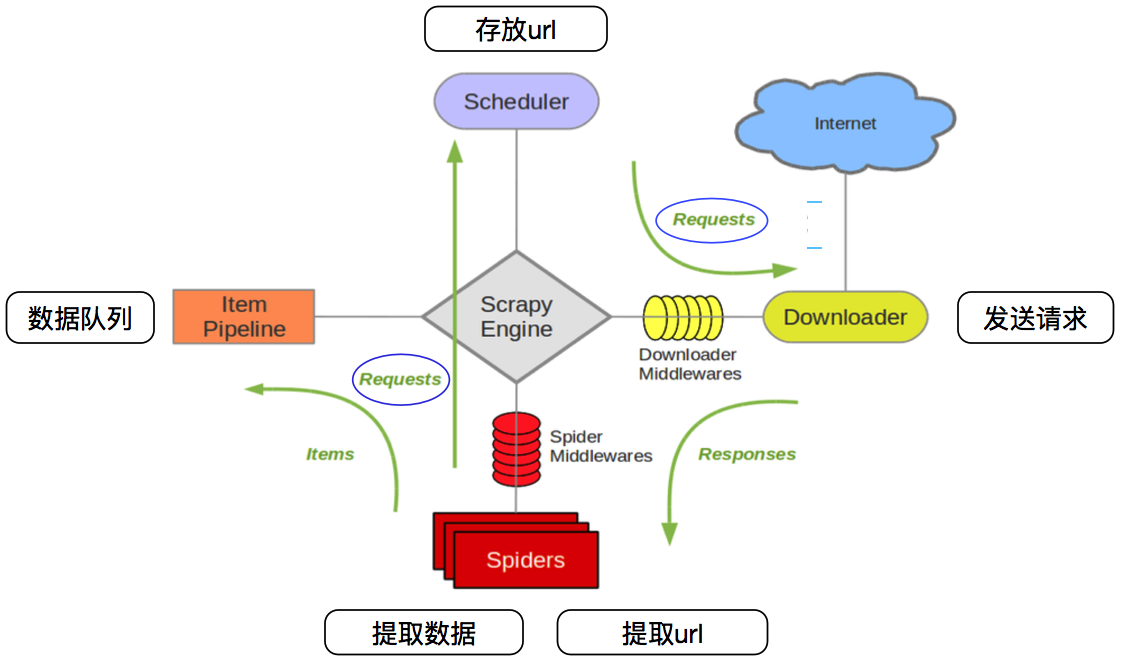
\includegraphics[width=0.85\textwidth]{figures/scrapy_introduction.png}
\caption{Scrapy 结构介绍} 
\end{figure}

3. 调度器(Scheduler)

在Scrapy框架中,调度器负责接收引擎发送过来的请求,并将这些请求压入请求队列中。调度器类似于一个URL的优先级队列,它决定了下一个要抓取的网址是什么,可以根据一定的规则和算法来确定抓取顺序,如优先级、深度优先、广度优先等。同时,调度器还负责去重,即在接收到请求后,会判断该网址是否已经在队列中,避免重复抓取相同的内容。在引擎再次请求时,调度器会从队列中取出下一个要抓取的网址并返回给引擎,以供下载器下载。调度器的主要作用是协调和管理请求的发送和处理,确保爬虫能够按照预期的方式运行。

4. 项目管道(Item Pipeline)

在Scrapy框架中,项目管道则是主要负责对爬取到的数据进行处理和持久化,包括清理、验证、存储到数据库等操作。当Spider解析完网页并提取出数据后,这些数据会被送入项目管道,然后依次经过管道中的不同组件进行处理,最终将处理后的数据存储到指定的位置。项目管道可以实现一系列功能,如数据清洗、去重、验证、转换格式、存储到数据库等,用户可以根据自己的需求自定义管道组件。我们就是在管道处,实现了对数据库的写入操作。

5. 中间件(Middlewares)

Spider 中间件是 Scrapy 框架中用于处理 Spider 与引擎之间交互的一种机制,可以对 Spider 生成的请求和从引擎返回的响应进行全局性的控制和处理,提高了爬虫的灵活性和可扩展性。在 Scrapy 中有两种类型的中间件:下载器中间件和 Spider 中间件。

Spider 中间件主要用于处理 Spider 类与引擎之间的交互,包括了 Spider 类生成的请求和从引擎返回的响应。通过 Spider 中间件,开发者可以处理请求前或处理响应后执行一系列的预处理或后处理操作,如对请求和响应进行加工、过滤、记录日志等。Spider中间件会用于实现一些通用的功能,如自定义请求头、添加代理、处理异常等,使得Spider类可以专注于数据解析和处理,而中间件负责处理请求和响应的其他逻辑。而下载器中间件是Scrapy框架中另一种类型的中间件,用于处理引擎和下载器之间的交互。下载器中间件主要负责处理从引擎传到下载器的请求和从下载器传到引擎的响应。

\begin{table}[h]
\centering
\begin{tabular}{@{}lll@{}}
\toprule
\textbf{组件} & \textbf{功能介绍} & \textbf{实现方式} \\ 
\midrule
Scrapy Engine & 负责数据的传递 & scrapy已经实现 \\
Scheduler & 队列存放request请求 & scrapy已经实现 \\
Downloader & 下载requests请求返回给引擎 & scrapy已经实现 \\
Spider & 处理引擎发来的response & 一般需要手搓 \\
Item Pipeline & 处理引擎传过来的数据 & 一般需要手搓 \\
Downloader Middlewares & 自定义的下载扩展 & 一般不用手写 \\
Spider Middlewares & 可以自定义请求和进行过滤 & 一般不用手写 \\
\bottomrule
\end{tabular}
\caption{Scrapy 组件功能介绍}
\label{tab:scrapy_components}
\end{table}

\subsection{爬虫主程序的设计}

创建好 Scrapy 的框架后,首先实现爬虫类的主要逻辑。我们设计的这个爬虫主要用于采集微博推文数据,根据指定的关键词和时间段进行搜索。第一个创建任务的节点会创建一个请求队列,然后会从 Redis 的请求队列中获取待爬取的 URL,并发送请求获取网页内容。爬虫程序解析网页内容,提取推文信息,并将结果保存到数据结构中。同时,程序也支持分页爬取,并且可以处理长推文和视频内容,还包含了一些辅助方法,用于解析 URL、时间和用户信息等等。

首先,为了实现分布式爬取微博的推文,我们需要将目的 url 插入到请求队列当中,之后的每一个爬虫节点要进去爬取时,从这个请求队列中 pop 出一个 url 进行处理。经过对微博信息进行一定的挖掘之后,设计了如下的函数,获取指定时间和关键词的推文。
\begin{minted}[bgcolor=gray!20, style=vs, fontsize=\footnotesize, fontfamily=tt, escapeinside=||]{python}  
    def add_urls_to_redis(self):
        """
        将待爬取的 URL 添加到 Redis 的请求队列中
        """
        ####### 清理过滤重复 Redis 队列的步骤  ########
        self.keywords = ['今天天气真好']
        
        # 这里的时间可替换成实际需要的时间段
        start_time = datetime.datetime(year=2024, month=6, day=10, hour=0)
        end_time = datetime.datetime(year=2024, month=6, day=11, hour=23)
        # 是否按照小时划分
        is_split_by_hour = True    
        urls = [ ]
        for keyword in self.keywords:
            if not is_split_by_hour: # 非按小时划分
                _start_time = start_time.strftime("%Y-%m-%d-%H")
                _end_time = end_time.strftime("%Y-%m-%d-%H")
                url = f"https://s.weibo.com/weibo?q={keyword}&
                        timescope=custom%3A{_start_time}%3A{_end_time}&page=1"
                urls.append(url)
            else: # 按小时划分
                time_cur = start_time
                while time_cur < end_time:
                    _start_time = time_cur.strftime("%Y-%m-%d-%H")
                    _end_time = (time_cur + datetime.timedelta(hours=1)).strftime("%Y-%m-%d-%H")
                    url = f"https://s.weibo.com/weibo?q={keyword}&
                            timescope=custom%3A{_start_time}%3A{_end_time}&page=1"
                    urls.append(url)
                    time_cur = time_cur + datetime.timedelta(hours=1)     
        ####### 将 URL 添加到请求队列中 ########
\end{minted}

设计入口函数,每个节点都从请求队列中获取一条 url 加载,实现了分布式爬虫。设计的逻辑是在方法开始时,调用上面讲到的方法,将待爬取的 URL 添加到请求队列中。然后使用一个无限循环 while True,不断地从 Redis 队列中取出 URL 进行爬取。使用 lpop 方法从 Redis 队列中获取队首的 URL,如果队列不为空,则返回 URL,否则返回 None。如果获取到了 URL,则使用 yield 关键字返回一个 scrapy.Request 对象,发送请求并指定回调函数为 parse 方法,即将爬取到的页面交给 parse 方法进行解析。

\begin{minted}[bgcolor=gray!20, style=vs, fontsize=\footnotesize, fontfamily=tt, escapeinside=||]{python}  
    def start_requests(self):
        """
        爬虫入口
        """
        # 将URL添加到Redis队列中
        self.add_urls_to_redis()
        # 开始爬取
        while True:
            # 从Redis队列中取出URL进行爬取
            url = self.rc.lpop('weibo_comment:start_urls')
            if url:
                # url = url.decode('utf-8')
                yield Request(url, callback=self.parse)
\end{minted}

设计爬虫的解析方法,首先我们从 response 中提取页面的 HTML 内容,并存储在变量 html 中。然后解析爬取到的网页内容,提取出微博信息块,获取微博详情页面的 url,并查找下一页的链接,以便继续爬取下一页的内容。

\begin{minted}[bgcolor=gray!20, style=vs, fontsize=\footnotesize, fontfamily=tt, escapeinside=||]{python}  
    def parse(self, response, **kwargs):
        """
        网页解析
        """
        html = response.text
        if '<p>抱歉,未找到相关结果。</p>' in html:
            self.logger.info(f'no search result. url: {response.url}')
            return
        tweets_infos = re.findall('<div class="from"\s+>(.*?)</div>', html, re.DOTALL)
        for tweets_info in tweets_infos:
            tweet_ids = re.findall(r'weibo\.com/\d+/(.+?)\?refer_flag=1001030103_" ', tweets_info)
            for tweet_id in tweet_ids:
                url = f"https://weibo.com/ajax/statuses/show?id={tweet_id}"
                yield Request(url, callback=self.parse_tweet, meta=response.meta, priority=10)
        next_page = re.search('<a href="(.*?)" class="next">下一页</a>', html)
        if next_page:
            url = "https://s.weibo.com" + next_page.group(1)
            yield Request(url, callback=self.parse, meta=response.meta)
\end{minted}

分开处理长推文和短推文数据,设计考虑了两个解析方法,分别是 parse\_tweet 和 parse\_long\_tweet。这两种方法组合起来,可以用于爬虫解析微博页面中的推文数据(包括普通推文和长微博),并且将解析得到的数据传递给项目管道进行后续处理,写入到 Redis 分布式集群或者 json 文件中。做这一步的操作,是因为微博的长推文和短推文的存储方法是有差异的,针对不同的数据进行不同的处理是必要的,否则会丢失一些信息。

\begin{minted}[bgcolor=gray!20, style=vs, fontsize=\footnotesize, fontfamily=tt, escapeinside=||]{python}  
    def parse_tweet(self, response):
        """
        解析推文
        """
        data = json.loads(response.text)
        item = self.parse_tweet_info(data)
        # item['keyword'] = response.meta['keyword']
        if item['isLongText']:
            url = "https://weibo.com/ajax/statuses/longtext?id=" + item['mblogid']
            yield Request(url, callback=self.parse_long_tweet, meta={'item': item}, priority=20)
        else:
            yield item

    def parse_tweet_info(self, data):
        """
        解析推文数据
        """
        tweet = {### 解析推文信息 ###}
        ### 特殊类型的推文条目,有就添加进去 ####
        return tweet

    def parse_long_tweet(self, response):
        """
        解析长推文
        """
        data = json.loads(response.text)['data']
        item = response.meta['item']
        item['content'] = data['longTextContent']
        yield item
\end{minted}

\subsection{Middlewares 的配置}

创建好 Scrapy 的框架还有爬虫主程序之后,再对中间件进行配置。我们定义了一个名为 IPProxyMiddleware 的中间件类,用于在爬虫发起请求时添加代理IP。其中,fetch\_proxy 方法用于获取一个代理IP,你可以根据实际情况重写该方法以从代理池中获取IP。在 process\_request 方法中,如果成功获取到代理IP,则将其添加到请求的 meta 中,并设置请求的代理。

要注意的是,当前的 fetch\_proxy 方法返回的是 None,表示没有获取代理IP,因为微博没有很好的反爬策略(爬了一天都没问题),感觉风险比较小。如果有自己的代理IP池,也可以在这里编写逻辑来获取有效的代理IP,并返回其格式化后的字符串,形如 "ip:port" 形式的字符串,例如我给出的注释部分的代码 "12.34.1.4:9090"。

\begin{minted}[bgcolor=gray!20, style=vs, fontsize=\footnotesize, fontfamily=tt, escapeinside=||]{python} 
class IPProxyMiddleware(object):
    """
    代理IP中间件
    """
    @staticmethod
    def fetch_proxy():
        """
        获取一个代理IP
        """
        ip_port = None
        # ip_port = "12.34.1.4:9090"
        return ip_port

    def process_request(self, request, spider):
        """
        将代理IP添加到request请求中
        """
        proxy_data = self.fetch_proxy()
        if proxy_data:
            current_proxy = f'http://{proxy_data}'
            spider.logger.debug(f"current proxy:{current_proxy}")
            request.meta['proxy'] = current_proxy
\end{minted}         

\subsection{Pipeline 的配置}

在 Pipeline 中,我定义了两个 Scrapy Pipeline 类,用于处理爬虫爬取到的数据。这些 Pipeline 类的主要目的是将数据写入到不同的目标中,JsonWriterPipeline 负责将数据写入到 JSON 文件中,将每个 item 格式化成 JSON 格式,并写入到文件中。文件的命名规则为 "爬虫名\_当前时间.jsonl",并且每行是一个 JSON 对象,用于存储一个 item 的数据。在处理 item 时,还为每个 item 添加一个名为 crawl\_time 的字段,记录爬取的时间戳,结果会保留在 spider 文件夹下的 output 文件夹下。

RedisPipeline 用于将数据写入到 Redis 中。在 process\_item 方法中,它通过调用 get\_redis 方法连接到 Redis 数据库,并将 item 转换为 JSON 格式后写入到指定的 Redis 列表中。列表的键名是由爬虫名加上 :items 组成的,例如 weibo\_comment:items,此处使用的默认 Redis 连接信息是连接到本地主机 (127.0.0.1) 的端口号 6381,使用默认的数据库 0,将会基于 Redis 分布式集群进行写入数据的操作。

\begin{minted}[bgcolor=gray!20, style=vs, fontsize=\footnotesize, fontfamily=tt, escapeinside=||]{python} 
class JsonWriterPipeline(object):
    """
    写入json文件的pipline
    """

    def __init__(self):
        self.file = None
        if not os.path.exists('../output'):
            os.mkdir('../output')

    def process_item(self, item, spider):
        """
        处理item
        """
        if not self.file:
            now = datetime.datetime.now()
            file_name = spider.name + "_" + now.strftime("%Y%m%d%H%M%S") + '.jsonl'
            self.file = open(f'../output/{file_name}', 'wt', encoding='utf-8')
        item['crawl_time'] = int(time.time())
        line = json.dumps(dict(item), ensure_ascii=False) + "\n"
        self.file.write(line)
        self.file.flush()
        return item

class RedisPipeline:
    """
    将数据写入到Redis的Pipeline
    """

    def process_item(self, item, spider):
        """
        处理item,将数据写入到Redis
        """
        redis_conn = get_redis(host='127.0.0.1', port=6381, db=0)
        redis_key = f"{spider.name}:items"
        redis_conn.lpush(redis_key, json.dumps(dict(item), ensure_ascii=False))
        return item
\end{minted}        

\subsection{Settings 的配置}

在 Setting 文件中需要定义爬虫的一些基本设置、请求头、中间件和管道,首先指定了爬虫的名称和模块,设定不遵守 robots.txt 规则。然后设置了请求的 Cookie,这是我自己的微博 Cookie,用于模拟登录状态。设置了默认的请求头,指定了连接到 Redis 数据库的主机地址和端口号,如果需要多节点运行爬虫的话,这里的地址号和端口号需要修改。设置允许中断恢复,设置了并发请求数为16,设置了下载延迟,避免对目标网站造成过大压力,也是防止IP被封。

最后就是关于中间件和管道的设置,设置下载中间件使用自定义的 IPProxyMiddleware,用于处理代理 IP,然后设置数据处理管道,包括将数据写入 JSON 文件的 JsonWriterPipeline 和将数据写入 Redis 的 RedisPipeline,根据需要进行设置。

\begin{minted}[bgcolor=gray!20, style=vs, fontsize=\footnotesize, fontfamily=tt, escapeinside=||]{python} 
# -*- coding: utf-8 -*-
BOT_NAME = 'weibo_spider'
SPIDER_MODULES = ['weibo_spider']
NEWSPIDER_MODULE = 'weibo_spider'
ROBOTSTXT_OBEY = False

DEFAULT_REQUEST_HEADERS = {
    'User-Agent': 'Mozilla/5.0 (Macintosh; Intel Mac OS X 10.13; rv:61.0) 
        Gecko/20100101 Firefox/61.0', Safari/537.36",
    'Cookie': "xxxx"
}

# 指定Redis连接信息
REDIS_HOST = 'localhost'
REDIS_PORT = 6379

# 允许中断恢复
SCHEDULER_PERSIST = True
CONCURRENT_REQUESTS = 16
DOWNLOAD_DELAY = 1

DOWNLOADER_MIDDLEWARES = { # 设置项目的中间件
    'scrapy.downloadermiddlewares.cookies.CookiesMiddleware': None,
    'scrapy.downloadermiddlewares.redirect.RedirectMiddleware': None,
    'weibo_spider.middlewares.IPProxyMiddleware': 100,
    'scrapy.downloadermiddlewares.httpproxy.HttpProxyMiddleware': 101,
}

ITEM_PIPELINES = { # 设置项目的管道优先级
    # 'weibo_spider.pipelines.JsonWriterPipeline': 300,
    'weibo_spider.pipelines.RedisPipeline': 299,
}
\end{minted}   

总结这部分的内容,这是一个基于 Scrapy 的爬虫,通过关键词搜索微博推文数据。通过使用 Redis 进行任务调度,利用集群存储爬取的 URL,支持按照设定的时间段和关键词进行搜索。程序通过解析响应页面,提取微博推文的相关信息,包括推文内容、发布时间、地理位置、转发数、评论数、点赞数等,支持对长微博进行完整内容的抓取。


\newpage
\section{Redis 集群结构与搭建}

Redis 是一个开源的、内存中的数据结构存储系统,它可以用作数据库、缓存和消息中间件。Redis 支持多种类型的数据结构,如字符串、哈希、列表、集合、有序集合等类型,并且提供了这些类型的丰富操作命令。Redis 是基于内存存储的,将数据存储在内存中,读写速度非常快,通常用于需要高性能读写的场景。同时其数据类型丰富,支持多种数据类型,也具有持久化的特点,将数据保存到磁盘上,可以通过 RDB(快照)或 AOF(追加式文件)两种方式来实现数据的持久化。

在这部分,我们最重要的是用到了其的分布式,Redis 支持通过分片(sharding)来实现水平扩展,也可以使用 Redis 集群(Redis Cluster)来自动管理分片。在进行排名的过程中,我们也使用了 Redis 提供的发布/订阅功能,使用消息队列和通知系统对所有的节点进行通知,让各个节点明白自己的任务是什么,并且通过接收所有节点的处理数据,再归并所有的排序结果输出。

Redis集群主要有三种方式:主从复制、哨兵模式和 Redis Cluster 集群模式。

\subsection{主从复制}

主从复制的部署相对简单,并且能有效地实现读写分离,提高系统的可用性和性能。在从节点(slaves)上,读操作的请求可以被路由,从而允许从节点直接读取主节点(master)的数据副本。在主从复制期间,主节点和从节点通常以非阻塞的方式运行,这意味着在数据库节点同步数据的过程中,主节点仍然能够及时地处理用户的插入、更新或删除操作,而不会影响到正常的业务处理。

但是主从复制也存在一些的缺点,在主节点崩溃期间,需要手动切换主机,同时会有部分数据不能及时同步到从服务器,造成数据不一致。或者 Slave 宕机崩溃后,多个Slave恢复时,大量的 SYNC 同步会造成 Master的 IO 压力迅速的增大。

\begin{figure}[H]
\centering
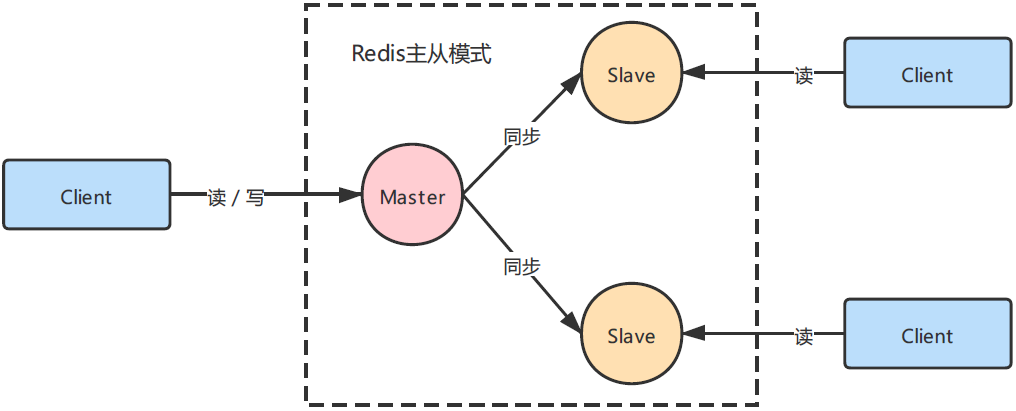
\includegraphics[width=0.85\textwidth]{figures/redis_master_slave.png}
\caption{Redis 主从复制简单图示} 
\end{figure}

\textbf{我们实现的分布式是基于 Redis 集群的,然后集群的工作原理又涉及到主从复制框架,所以在这部分我们详细介绍一下主从复制。}主从复制主要是由 Redis 的 replicaof 模块实现的,可以实现节点的读写分离、容灾恢复、数据备份以及水平扩容支撑高并发。下面介绍一下工作的流程,一般来说主从复制有两种实现方式,一种是全量复制,另一种是增量复制,各有优缺点,我们介绍全量复制,全量复制相当于就是做了一个备份,对空间的要求会比较大但是比较简单。

在正常工作的情况下,假设我们有两个实例如图3,其中一个为主实例(port:6379),另一个为从实例(port:6382),第一步由于从实例没有一点主实例的信息,所以进行 SYNC 同步。如果从库是因为断网等原因导致需要重新更新数据,这时候在从库里有主库的信息,则从库给主库发送 PSYNC (部分全同步)命令,表示要重新进行数据同步,主库会根据这个命令的参数来启动复制数据;第二步,主库向从库发送 FULLRESYNC 响应命令并带上了之前的两个参数(主库 runID 和主库目前的复制进度 offset);

之后第三步,主库执行 bgsave 命令,生成Redis数据备份文件,也被叫做Redis数据快照,发送给从库,从库接收到 RDB 文件后,会先清空当前数据库,然后加载 RDB 文件,这是因为从库在通过 replicaof 命令开始和主库同步前,可能保存了其他数据,为了避免之前数据的影响,从库需要先把当前数据库清空。最后一步是主实例将发送过程中收到的指令存储到 replication buffer 中,并发送给从库,后续主库接收到的写命令都会被主库传递给所有从库,以保证数据的一致性。

\begin{figure}[H]
\centering
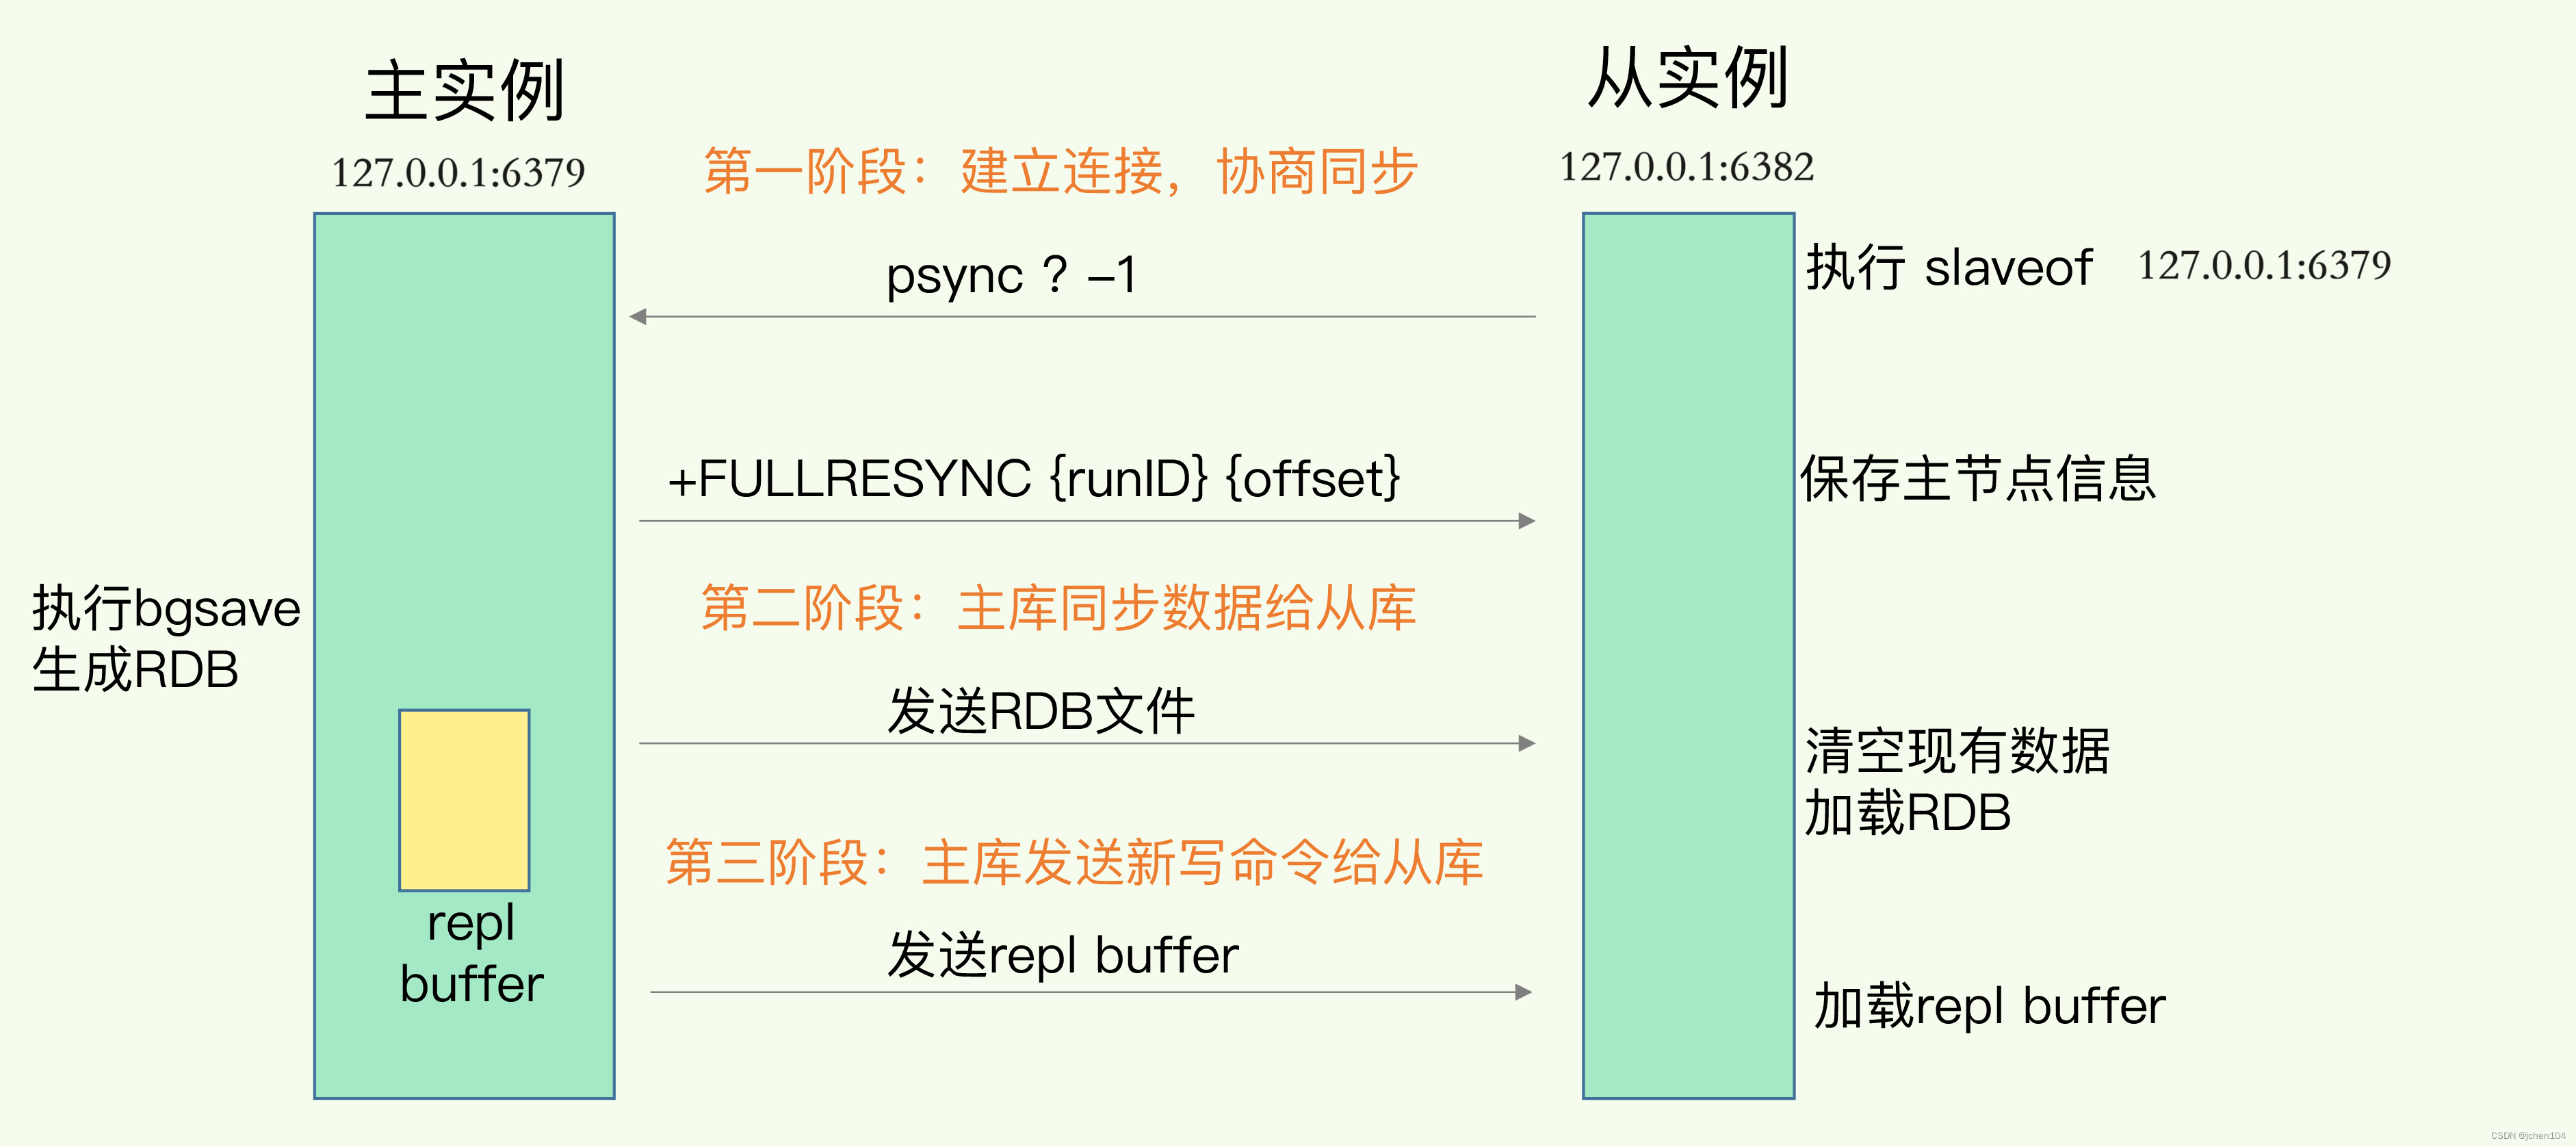
\includegraphics[width=1\textwidth]{figures/master-slave.png}
\caption{Redis 主从复制部分全同步详细流程} 
\end{figure}

\subsection{Redis 集群部署}

Redis 集群是由多个 Redis 服务器组成的分布式数据库服务集群,集群之中有多个Master主节点,每一个主节点都可读可写。节点之间会互相通信,两两相连,此外Redis集群无中心节点,在Redis-Cluster集群中,可以给每一个主节点添加从节点,主节点和从节点直接遵循主从复制模型的特性。我们搭建了一个三主三从的集群模式(图5):

\begin{figure}[H]  
    \centering  
    \begin{minipage}{0.48\textwidth}  
        \centering  
        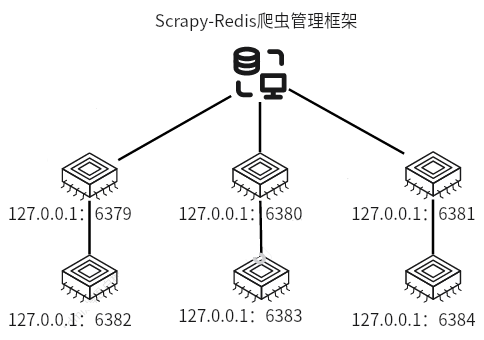
\includegraphics[width=\textwidth]{figures/redis-cluster.png}  
        \caption{Redis 主从结构示意}  
    \end{minipage}  
    \hfill % 这是一个水平填充命令,用于在两个minipage之间添加一些间距  
    \begin{minipage}{0.48\textwidth}  
        \centering  
        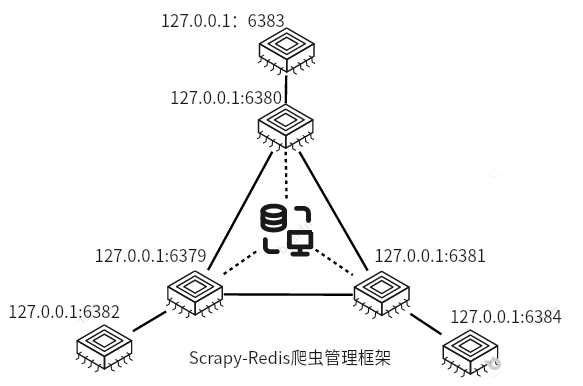
\includegraphics[width=\textwidth]{figures/redis-cluster2.png}  
        \caption{Redis 集群结构示意}  
    \end{minipage}  
\end{figure} 

其中端口号为6379、6380、6381的为主节点,6382、6383、6384分别对应上述几个主节点的从节点。对比搭建多个相互独立主从的数据库(图4),搭建数据库集群(图5)的最主要优势是高可用性和负载均衡性,确保即使某个节点发生故障,整个集群仍然能够继续运行,同时数据库集群能够自动实现负载均衡,确保数据请求被均匀地分配到各个节点上,从而避免单个节点过载,提高整体性能。

搭建 Redis 集群,我们复制了多个 Redis 数据库的客户端,配置每个客户端的的IP和端口号,使用一台主机的不同端口号来模拟分布式情况,设置了三台主库和三台从库,三台主库之间实现了集群管理,从库会在主库崩溃后代替主库的位置进行运行。修改配置文件,使用批处理命令使用自定义的配置文件来运行所有的数据库的客户端,如下。

% \begin{figure}[H]
% \centering
% 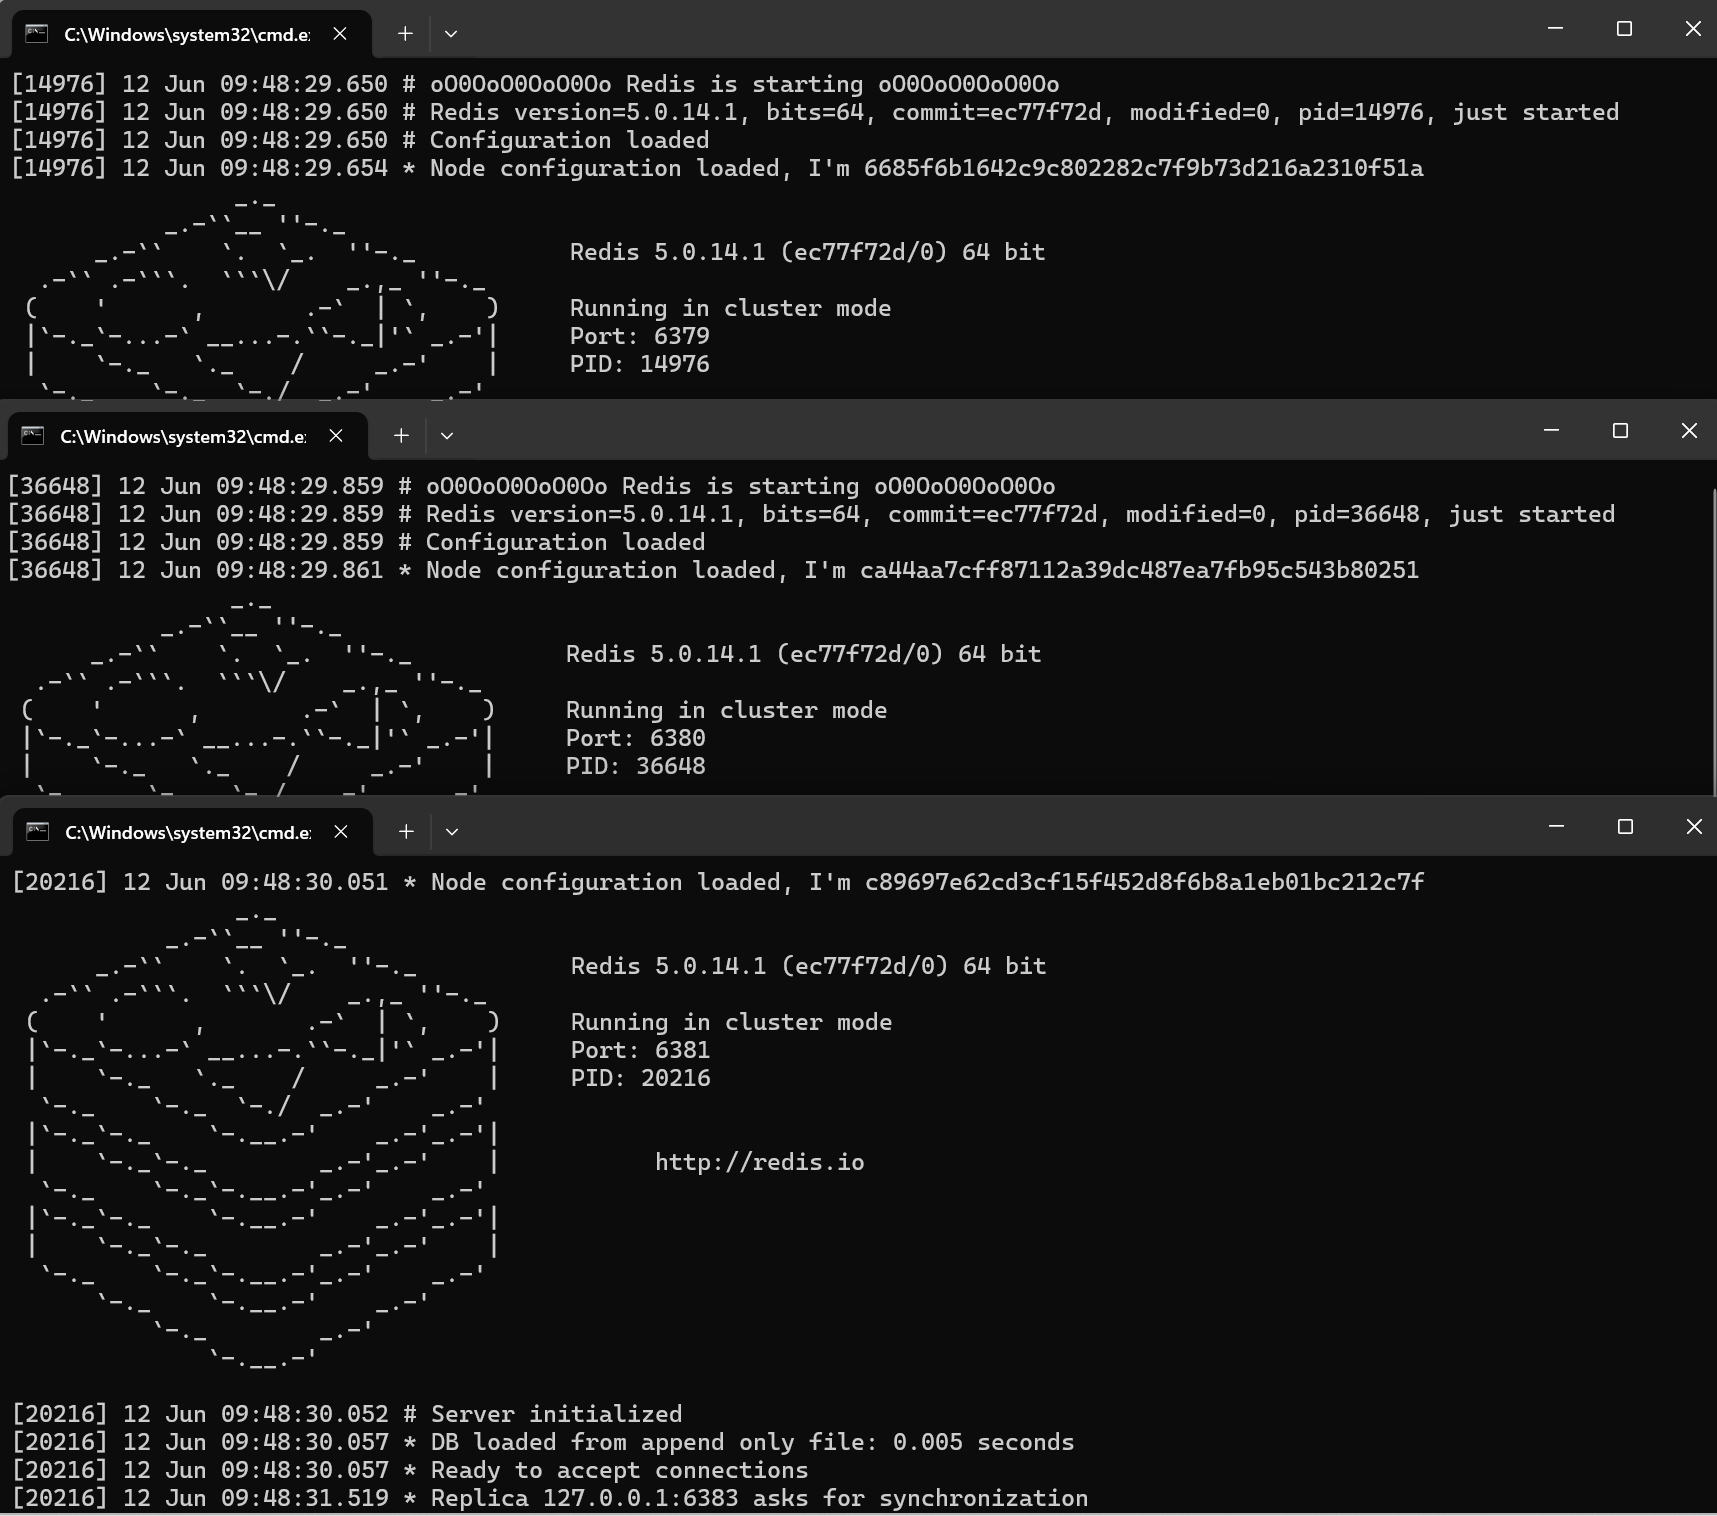
\includegraphics[width=0.85\textwidth]{figures/masters.png}
% \caption{Redis 主从复制简单图示} 
% \end{figure}

\begin{figure}[H]  
    \centering  
    \begin{minipage}{0.495\textwidth}  
        \centering  
        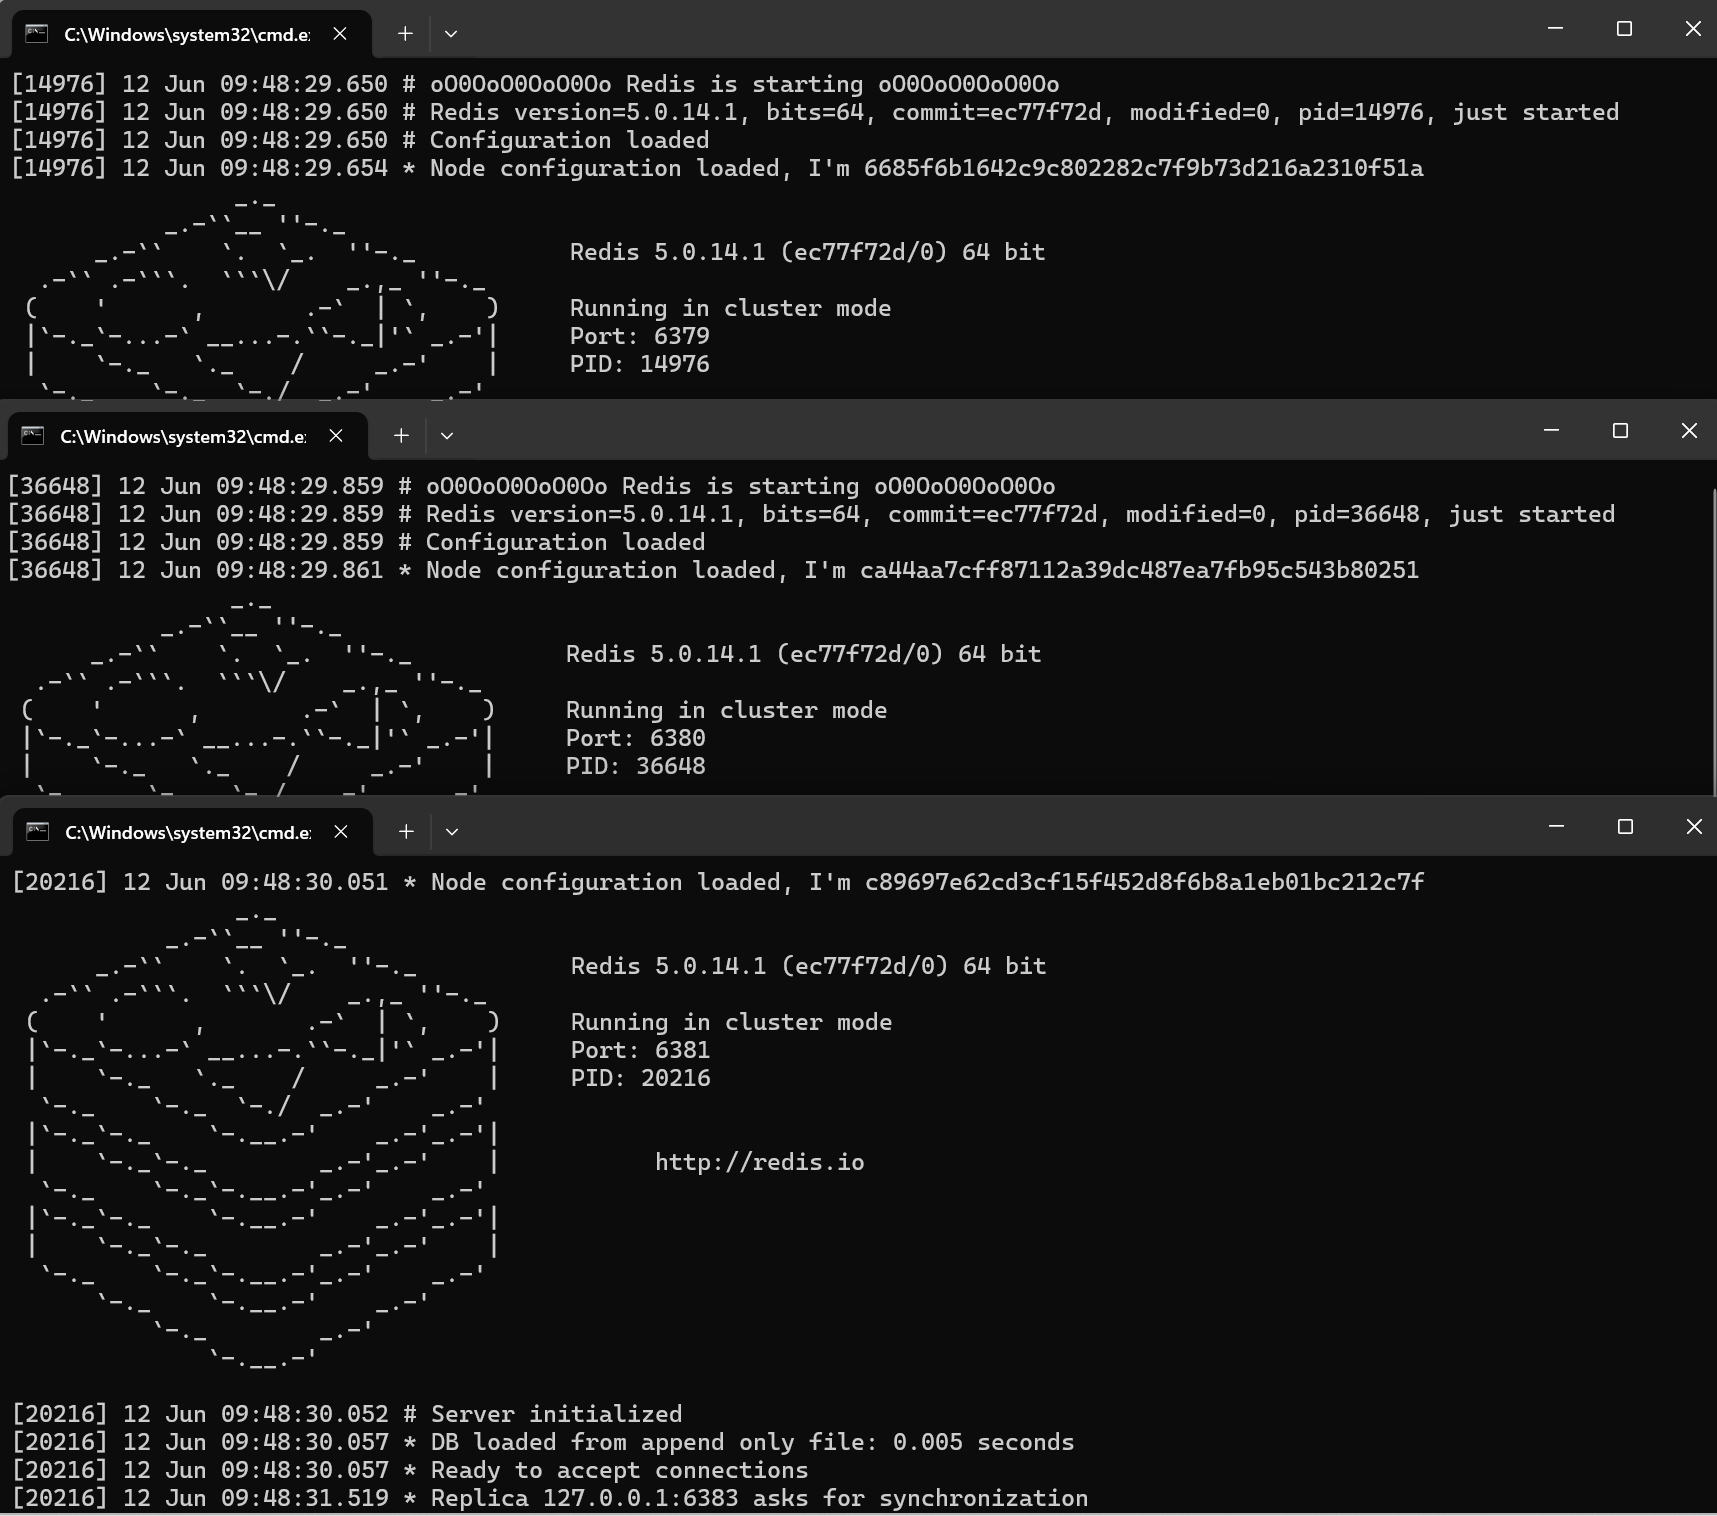
\includegraphics[width=\textwidth]{figures/masters.png}  
        \caption{主节点运行情况}  
    \end{minipage}  
    \hfill % 这是一个水平填充命令,用于在两个minipage之间添加一些间距  
    \begin{minipage}{0.495\textwidth}  
        \centering  
        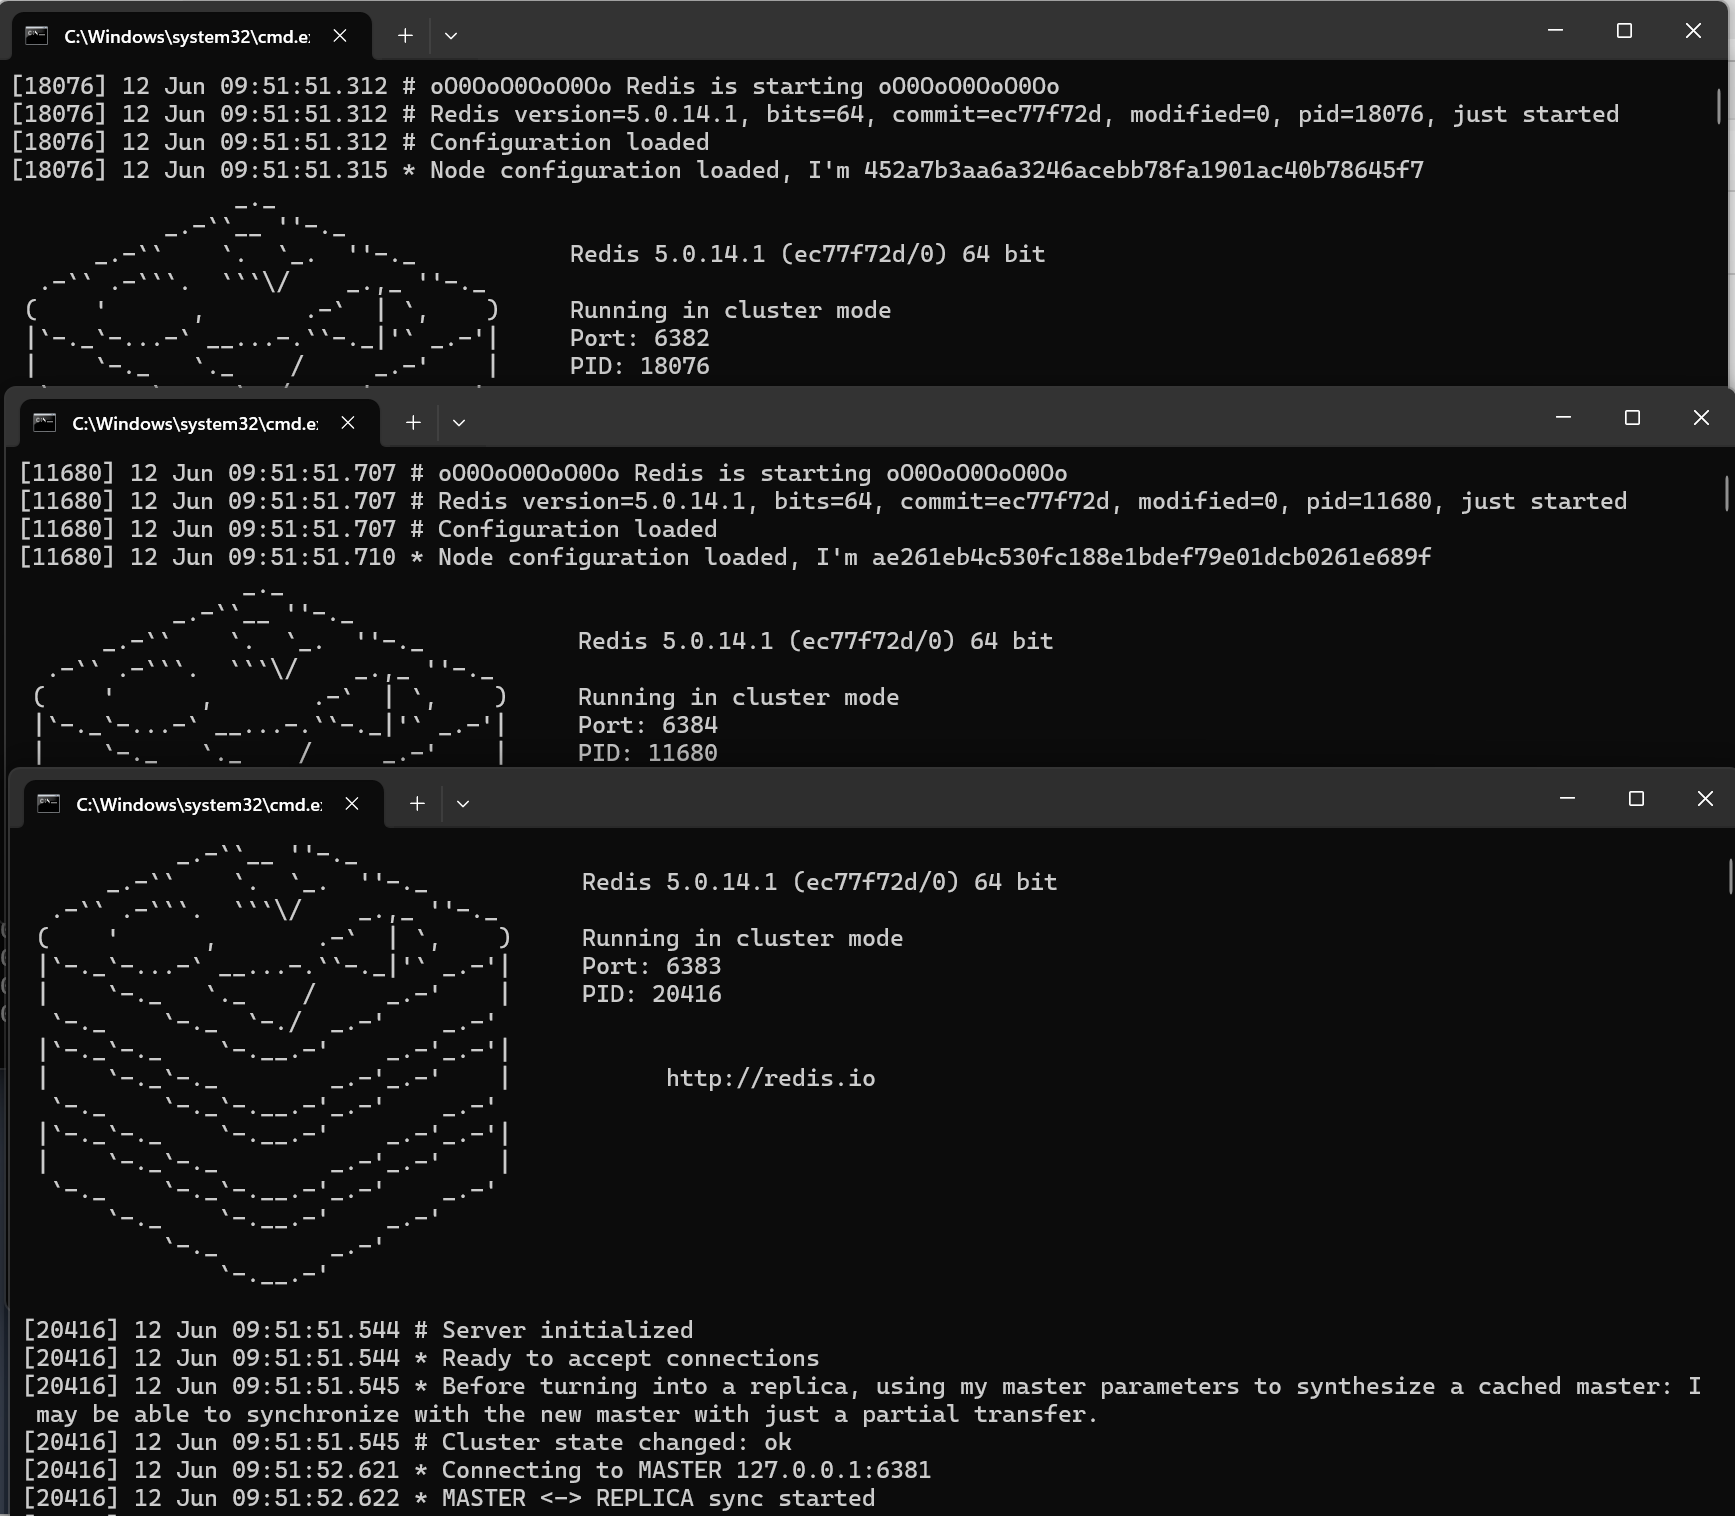
\includegraphics[width=\textwidth]{figures/slaves.png}  
        \caption{从节点运行情况}  
    \end{minipage}  
\end{figure} 

至此,我们完成了 Redis 集群的搭建,我们省去了大部分繁琐的配置操作过程,虽然跑代码没问题,但是主从关系和集群还存在一些关联性的问题,需要进一步的解决。

\subsection{节点的通信方式}

Redis Cluster节点间采取 Gossip 协议进行通信,每个节点都有一个专门用于节点通信的端口,用于交换信息(包括故障信息、增加减少节点的信息等)。同时,我们在爬虫系统中用到了远程的过程调用,目的是实现跨节点任务分配和分类数据收集。

\subsubsection{Redis 节点通信}

查阅 Redis 的说明文档,了解到集群内所有的消息都采用相同的消息头结构,它包含了发送节点关键信息,如节点id、槽映射、节点标识(主从角色, 是否下线)等,而消息体定义了发送消息的数据,其中 ping、meet、pong 都采用 cluster MsgDataGossip 数组作为消息体数据,实际消息类型使用消息头的 type 属性区分。接收节点收到 ping/meet 消息时,执行解析消息头和消息体流程主要有两部分:

\textbf{进行解析消息头的过程},消息头包含了发送节点的信息,如果发送节点是新节点且消息是meet类型,则加入到本地节点列表;如果是已知节点,则尝试更新发送节点的状态,如槽映射关系、主从角色等状态。

\textbf{进行解析消息体的过程},如果消息体的数组包含的节点是新节点,接收节点会尝试发起与该新节点的 meet 握手流程;如果是已知节点,接收节点则会去检查 flags 字段来确定该节点是否已下线,这有助于进行故障转移。

最后在消息处理完后回复pong消息,内容同样包含消息头和消息体,发送节点接收到回复的 pong 消息后,采用类似的流程解析消息并更新与接收节点最后通信时间。除了使用 Redis 自带的节点通信方式,我们还使用了远程过程调用,

\subsubsection{RPC 远程过程调用}

我们使用了 Redis 作为消息代理,基于分布式缓存和消息队列的方法,来对数据库数据进行排名计算。考虑使用 Redis 的 zset 数据结构来实现排名计算,因为它天然地支持排序和排名功能。此外我们\textbf{选择基于消息队列的方法,因为其灵活和可扩展}。通过消息队列,我们可以将任务异步地发送到不同的节点进行处理,从而实现并行处理和任务分发。另外,如果系统中有其他需要异步处理的任务,我们也可以利用同样的消息队列架构进行处理。\textbf{通过Redis的发布与订阅功能,实现了远程过程调用(RPC)的机制}。简单概括一下来说,就是在一个频道中发布了排名任务的描述,然后在另一个地方订阅这个频道,以便接收任务。

当一个任务被发布到 Redis 频道时,其他地方可以通过订阅该频道来接收到这个任务。这种模式允许不同的组件在系统中并行处理,使得它们可以独立地进行通信和处理任务。任务的发布者和接收者是不同的功能模块,它们是通过 Redis 频道进行通信的,我们可以任选排名任务的发布者。通过Redis Cluster 客户端,代码连接到 Redis 集群,并在集群中的不同节点上执行任务,然后返回汇总到程序中,再进行归并的排序。在数据量大的情况下,允许任务在多个节点上并行执行,提高了系统的性能和可伸缩性。

\newpage
\section{Streamlit 可视化交互页面}

Streamlit 是一个用 Python 编写的开源库,旨在帮助数据科学家快速创建数据驱动的 Web 应用程序。它的设计目标是让用户可以在几行代码内快速搭建可视化界面,展示数据分析结果,而无需深入了解 Web 开发。使用 Streamlit,可以轻松地将数据可视化、交互式组件和文本内容整合到一个简单的 Web 应用程序中。可以通过几行代码快速创建交互式组件,如滑块、复选框、下拉菜单等,与用户互动,同时也可以轻松地在本地运行应用程序,并且也很容易部署到各种平台,如云服务供应商或共享给其他人。

\subsection{搭建 Web 搜索页面}

设计代码利用 Streamlit 构建了一个简单的 Web 应用程序,用于连接和查询 Redis 数据库中的数据。首先通过侧边栏选择器提供了选项,包括选择查询请求发出的端口号、收集搜索关键词以及是否设置日期和页面数量。然后连接到Redis数据库,根据用户的选择查询相应的数据,并在页面上展示查询结果,最后关闭与 Redis 数据库的连接。通过这个应用程序,用户可以方便地查询和浏览 Redis 集群中的微博推文数据。

\begin{minted}[bgcolor=gray!20, style=vs, fontsize=\footnotesize, fontfamily=tt, escapeinside=||]{python} 
if __name__ == "__main__":
    # Streamlit应用程序
    st.title('Redis 数据库查询')
    st.sidebar.title("排名参数选择")

    # 左侧下拉菜单选择发布任务的端口号,添加下拉菜单以选择关键键
    # 选择是否进行分布式搜索
    # 设置日期的复选框,设置页面数量的复选框
    
    startup_nodes = [{"host": "127.0.0.1", "port": selected_port}]

    # 创建RedisCluster实例
    rc = RedisCluster(startup_nodes=startup_nodes, decode_responses=True)

    # 在Streamlit应用程序中调用查询函数
    query_redis_data(selected_key, number, begin_date)
    
    # 关闭连接
    rc.close()
\end{minted} 

\subsection{实现分布式排名}

基于消息队列和有序集合(zset)的 Redis 集群分布式排名是一种比较有效的解决方案,我们使用这个方案来用于在分布式环境中对数据进行排序和排名。

\subsubsection{排名任务发布}

我们在交互界面会选择一个端口号的 Redis 作为命令的发布者(也很常被定义为生产者),发布者将需要排序的数据信息作为消息发布到消息队列中。
每个节点从消息队列中获取数据,并将其存储在Redis集群中的有序集合(zset)中,这个zset中的成员是数据项,分数是需要排序的指标,比如评论数、创建时间等。

\begin{minted}[bgcolor=gray!20, style=vs, fontsize=\footnotesize, fontfamily=tt, escapeinside=||]{python} 
def enqueue_rank_task(rc, rank_key, number):
    try:
        # 发布排名任务到频道
        rc.publish(message)
        print("排名任务已发布到频道。")
    except ConnectionError as e:
        print("连接到 Redis 集群失败:", e)
\end{minted} 

\subsubsection{分布式排名计算}

每个节点获取到数据后,将数据存储在本地的有序集合(zset)中。每个节点上的数据只是部分数据,为了计算全局排名,需要使用分布式算法。我们使用的是简单的分布式归并排序,将每个节点收集到的有序集合进行归并,这些算法可以将每个节点上的有序集合合并成一个全局有序集合。

\begin{minted}[bgcolor=gray!20, style=vs, fontsize=\footnotesize, fontfamily=tt, escapeinside=||]{python} 
def distributed_rank_worker(rc, number):
    results = [ ]
    try:
        # 订阅排名频道
        pubsub = rc.pubsub()
        pubsub.subscribe('rank_channel')

        while True:
            # message = next(pubsub.listen())
            message = pubsub.get_message()
            if message:
                if message['type'] == 'message':
                    # 消息分解的过程省略
                    # 创建线程池
                    with ThreadPoolExecutor(max_workers=3) as executor:
                        # 提交并行任务
                        futures = [
                            executor.submit(execute_rank, rank_key, rc_6379),
                            executor.submit(execute_rank, rank_key, rc_6380),
                            executor.submit(execute_rank, rank_key, rc_6381)
                        ]
                        
                        # 等待所有任务完成
                        for future in futures:
                            result = future.result()  
                            results.append(result)

                    # 合并结果,进行归并排序
                    results = merge_sorted_lists(results, rank_key)
\end{minted} 

\subsubsection{查询排名结果}

客户端向任意一个Redis节点(由用户设置,也就是任务发布的节点)发送查询请求,该节点负责计算全局排名,并返回给客户端。这种方法的优势在于它可以横向扩展,通过添加更多的节点来处理更多的数据和请求,从而实现高性能和可扩展性。同时,我们也提供了灵活的排序方式,可以根据需要选择不同的指标进行排序,包括了评论数、还有推文创建时间。之前其实考虑过按照情感价值来进行排序,就是说建立一个情感词库,然后看推文中出现情感词库的词频来进行排名,结果效果很差很差,有可能是词库的问题(数据量小,没有找到数据来源),这里就删掉了不做介绍。

下面展示的是查询函数,涉及到了一些条件操作,返回排名前 number 的数据条目。

\begin{minted}[bgcolor=gray!20, style=vs, fontsize=\footnotesize, fontfamily=tt, escapeinside=||]{python}
def query_data(searchword, rankword, number, begin_date=None):
    """
    查询 Redis 中包含特定关键字的数据,返回排名前几名的数据列表
    """
    # 存储符合条件的数据
    filtered_data = []
    # 检索键对应的列表数据
    list_data = rc.lrange("weibo_comment:items", 0, -1)
    
    # 遍历列表中的每个字符串元素,并解析为 JSON 对象
    for json_string in list_data:
        data = json.loads(json_string)
        if searchword in data.get('content', ''):
            # 检查日期是否符合要求
            if begin_date:
                # 如果创建日期不为空且在指定日期之后,则加入筛选结果

    aim_tag = ["comments_count", "created_at",]
    if rankword in aim_tag:
        # 对符合条件的数据按照评论数进行排序,取前几名
    else:
        # 进行分布式搜索操作
    return top_data
\end{minted} 

\section{交互界面展示}

我们实现的项目是基于Scrapy-Redis的微博推文分布式爬虫,我们展示的可视化界面是一个基于 Streamlit 和 Redis 集群的微博推文数据查询工具,旨在帮助用户方便地查询和浏览存储在 Redis 数据库中的有排名的推文数据。

\begin{figure}[H]
\centering
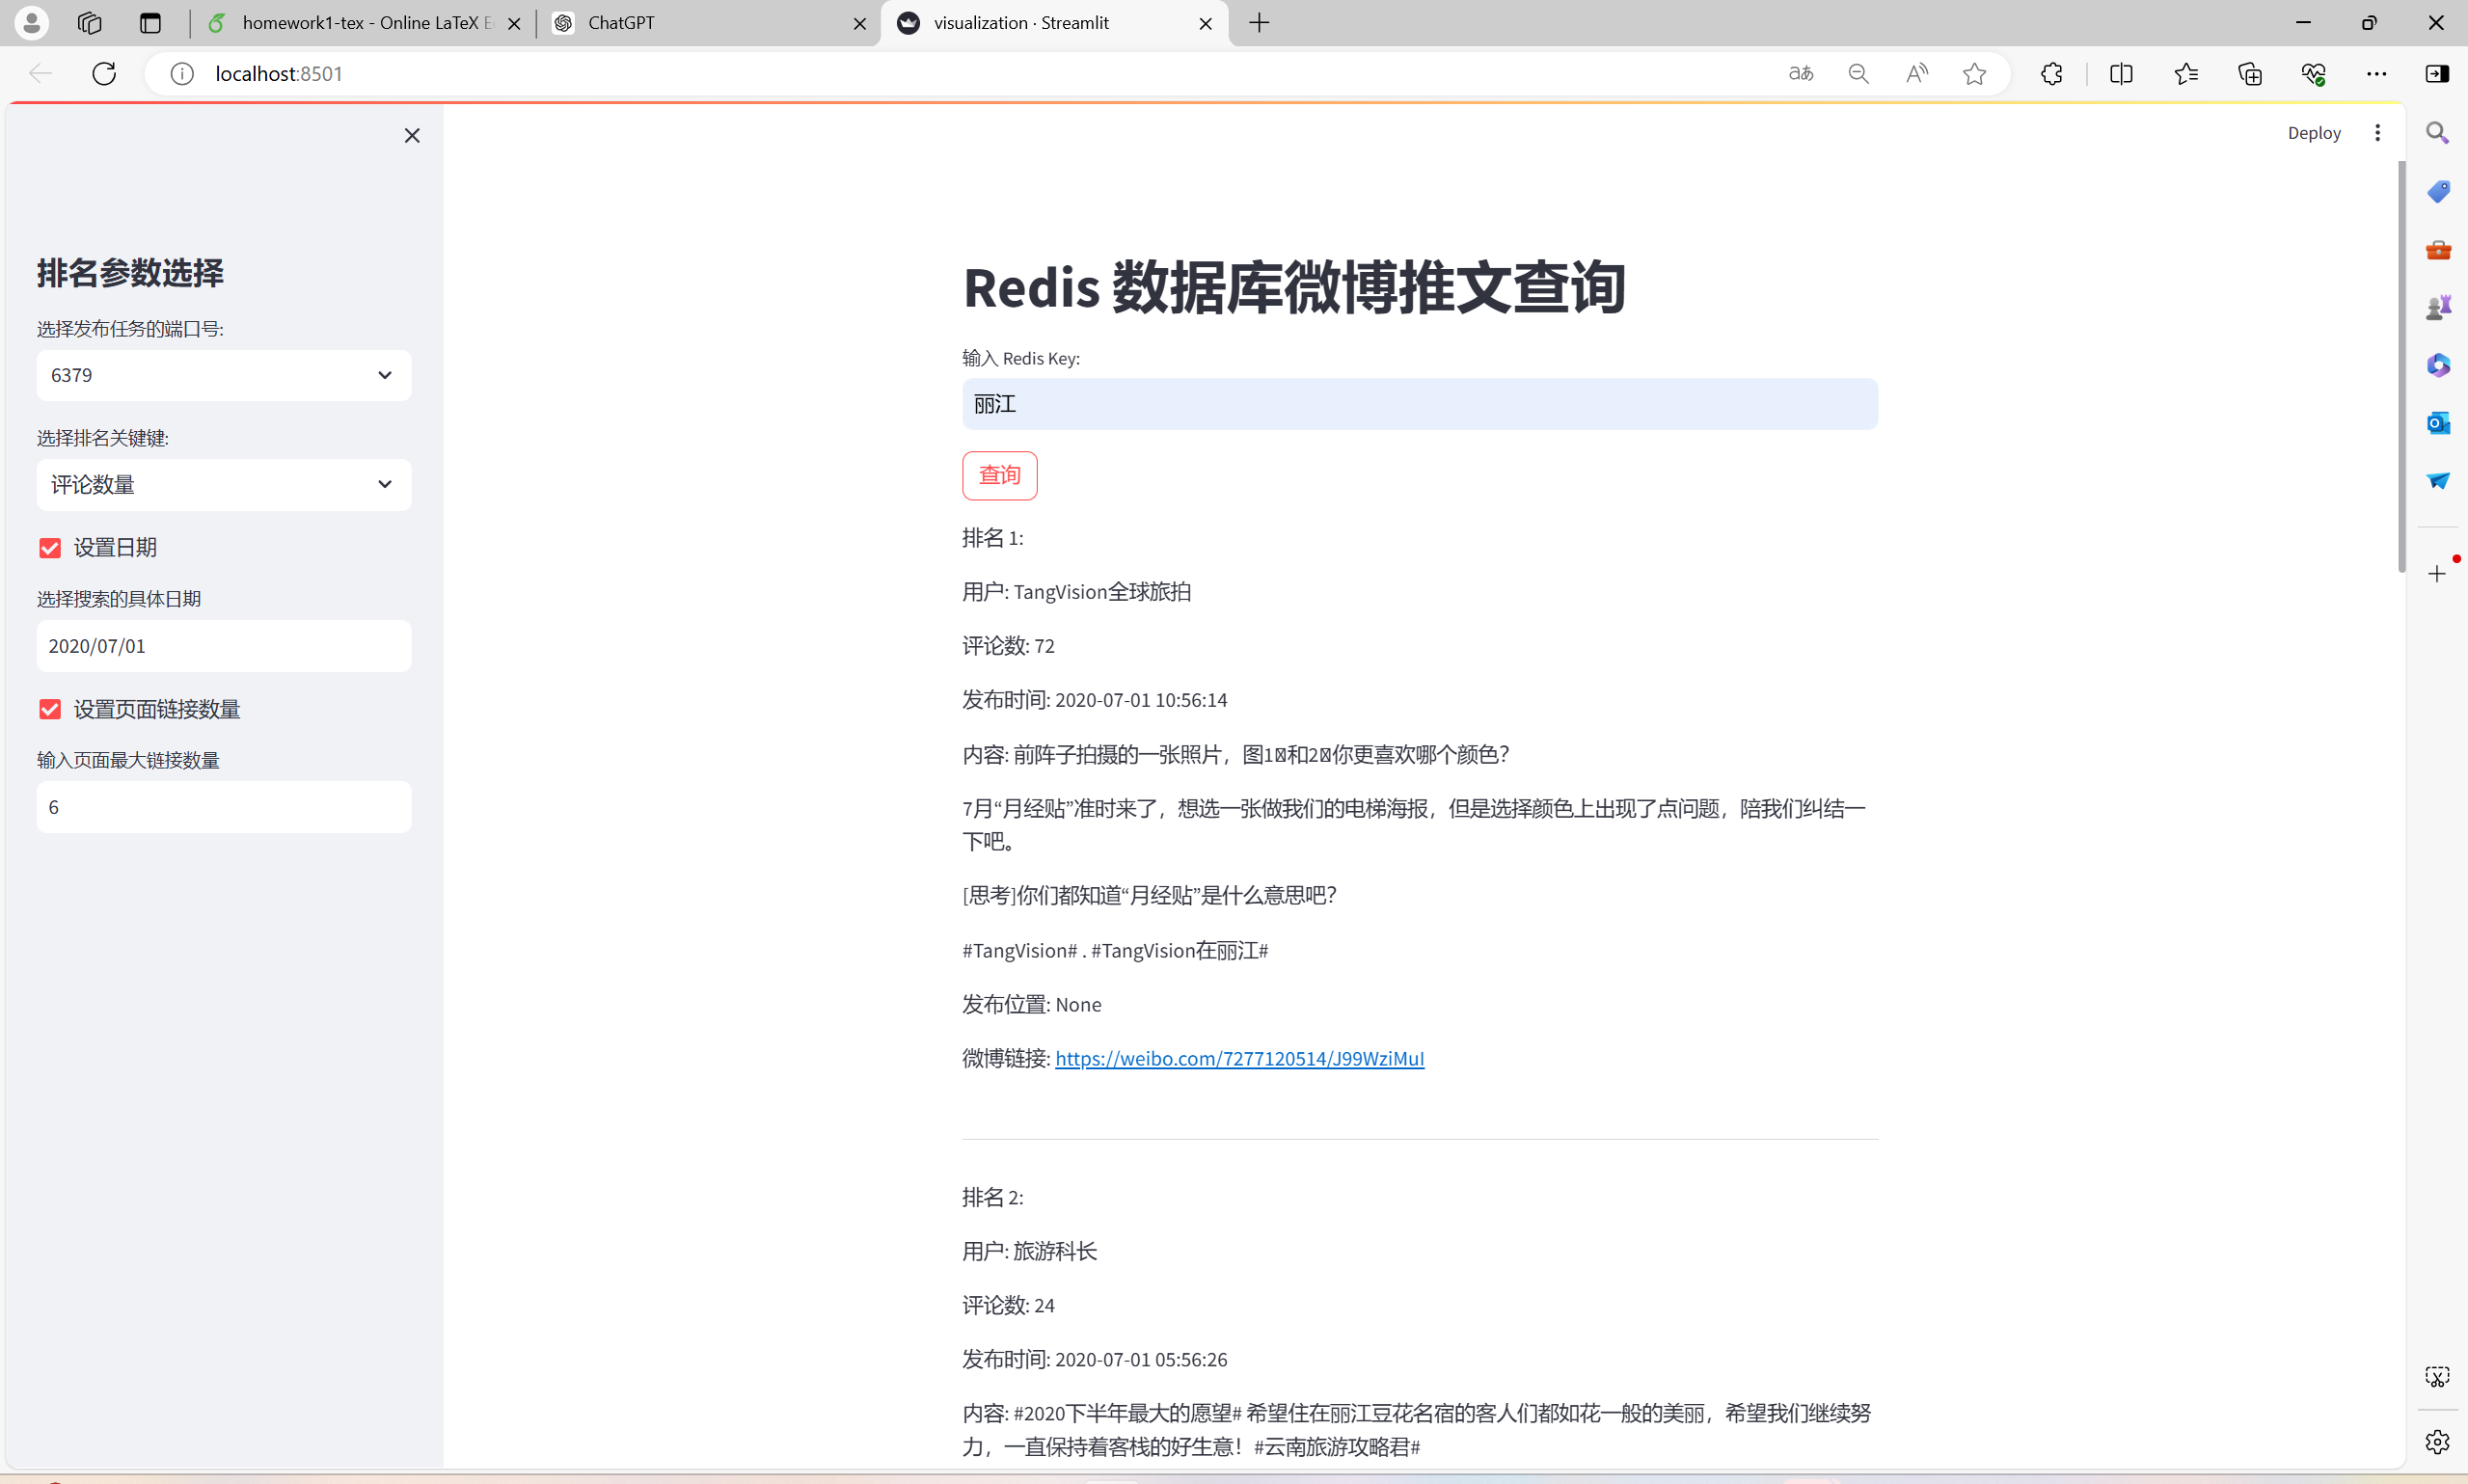
\includegraphics[width=1\textwidth]{figures/lijiang.png}
\end{figure}

\begin{figure}[H]
\centering
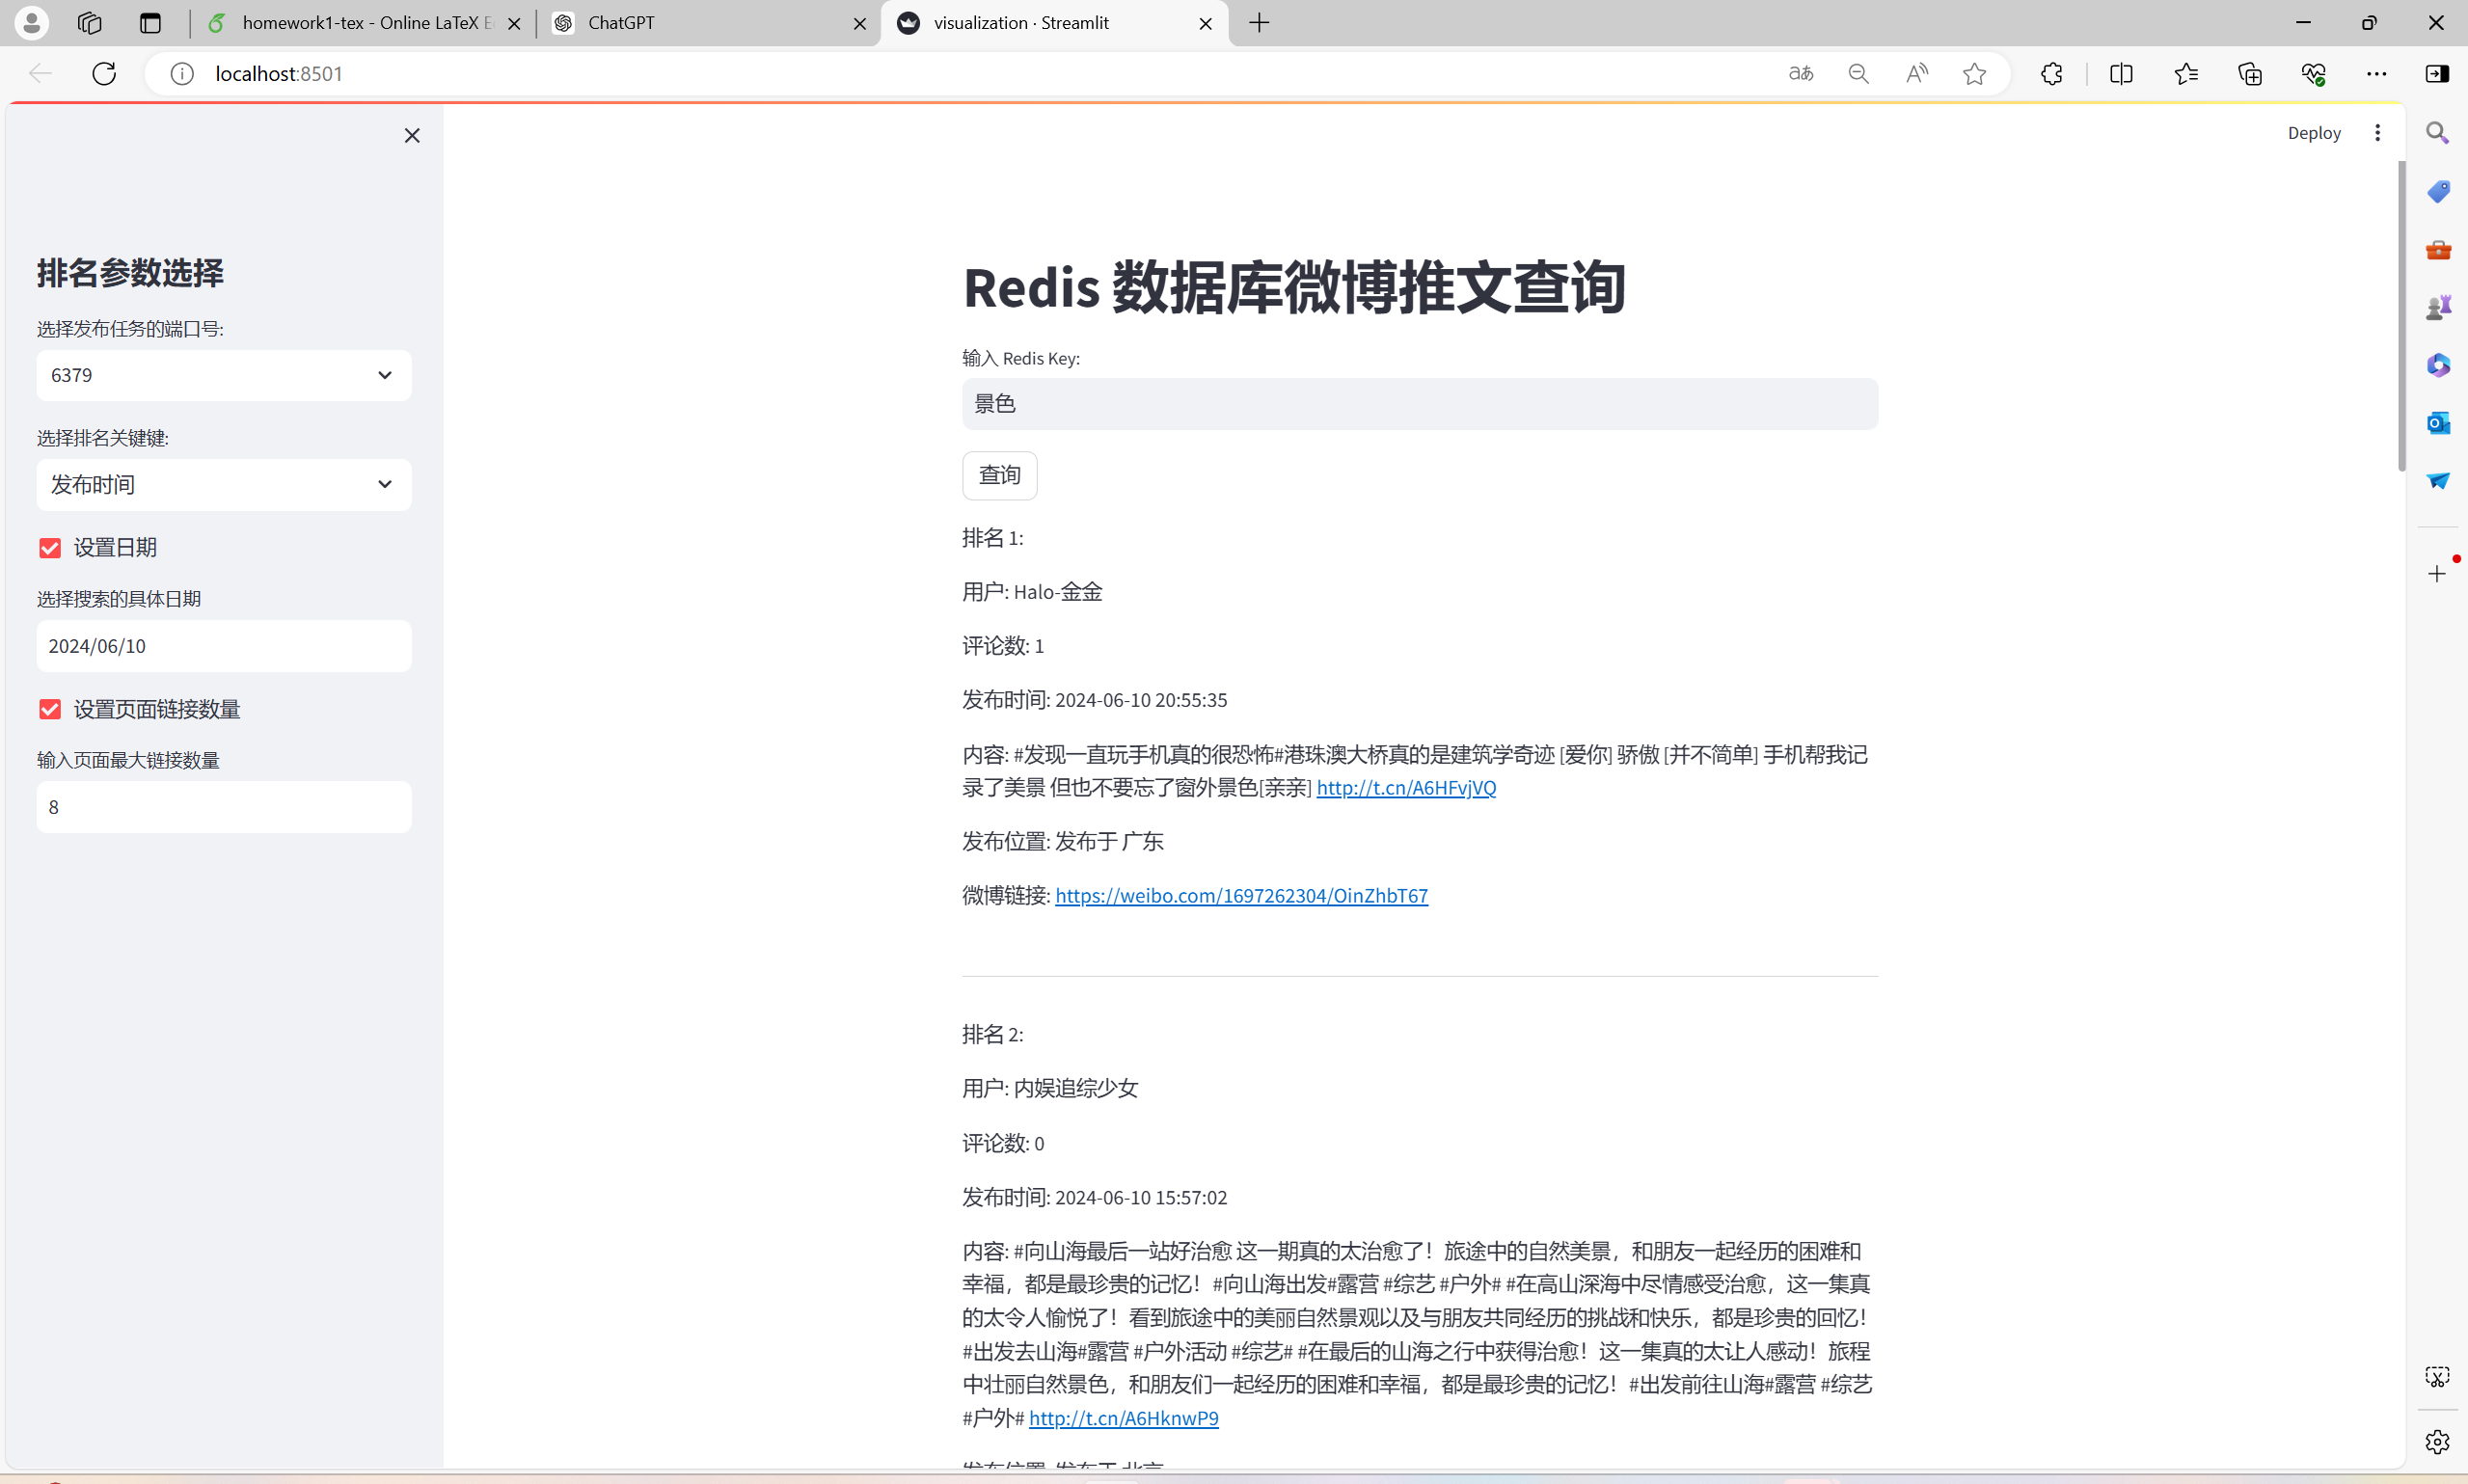
\includegraphics[width=1\textwidth]{figures/jingse.png}
\end{figure}

界面的左侧栏提供了各种选择器,用户可以根据自己的需求选择不同的排名参数和查询条件以及设置日期和页面链接数量。通过交互操作,用户可以轻松地查找和浏览符合条件的数据,并以清晰的格式展示在界面上。

下面展示的是集群的部署展示,如果需要测试,可以按照作业包文件中的部署格式,利用批处理文件一键启动,每个文件夹中通过配置文件运行Redis 服务器端。

\begin{figure}[H]
\centering
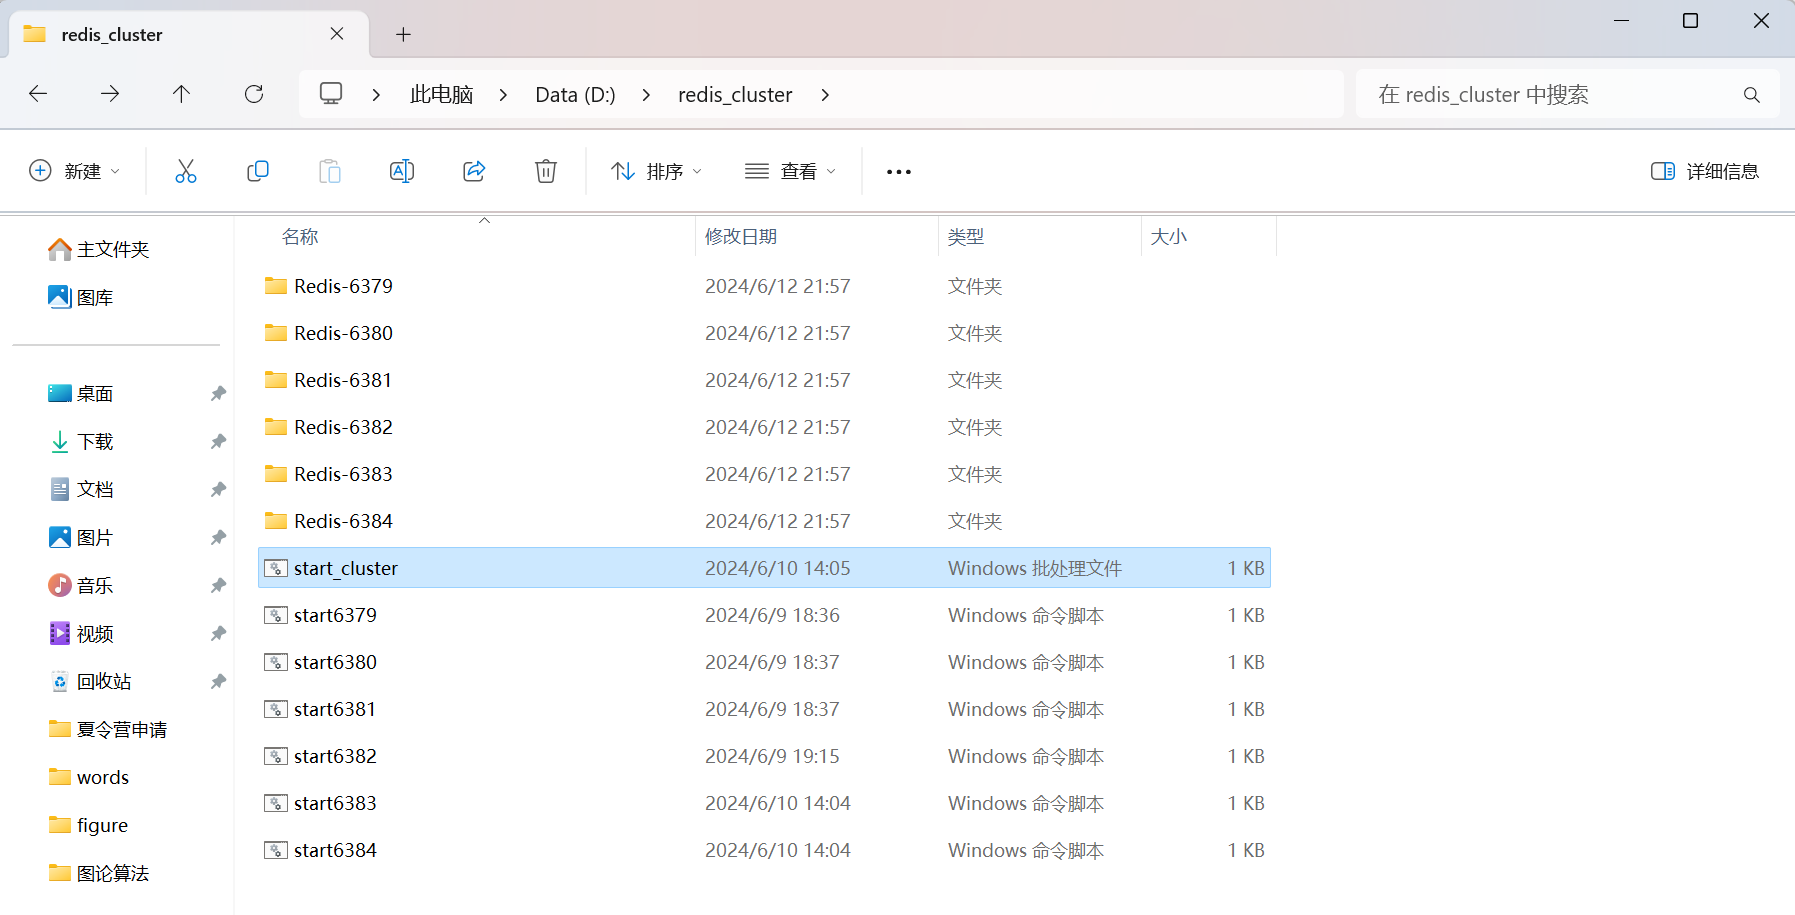
\includegraphics[width=1\textwidth]{figures/cluster.png}
\end{figure}

接下来展示的是通过 Redis Manager 中可视化的数据库集群的键值信息,可以发现在主节点6379、6380、6381中的信息是同步的,如果我们在其中一个节点插入信息,会自动重定向到目标存储主节点,这里用到的应该是对键名的哈希,然后再输入一次命令就可以进行写入,刷新数据库状态发现六个节点都能看到新插入的数据。

\begin{figure}[H]
\centering
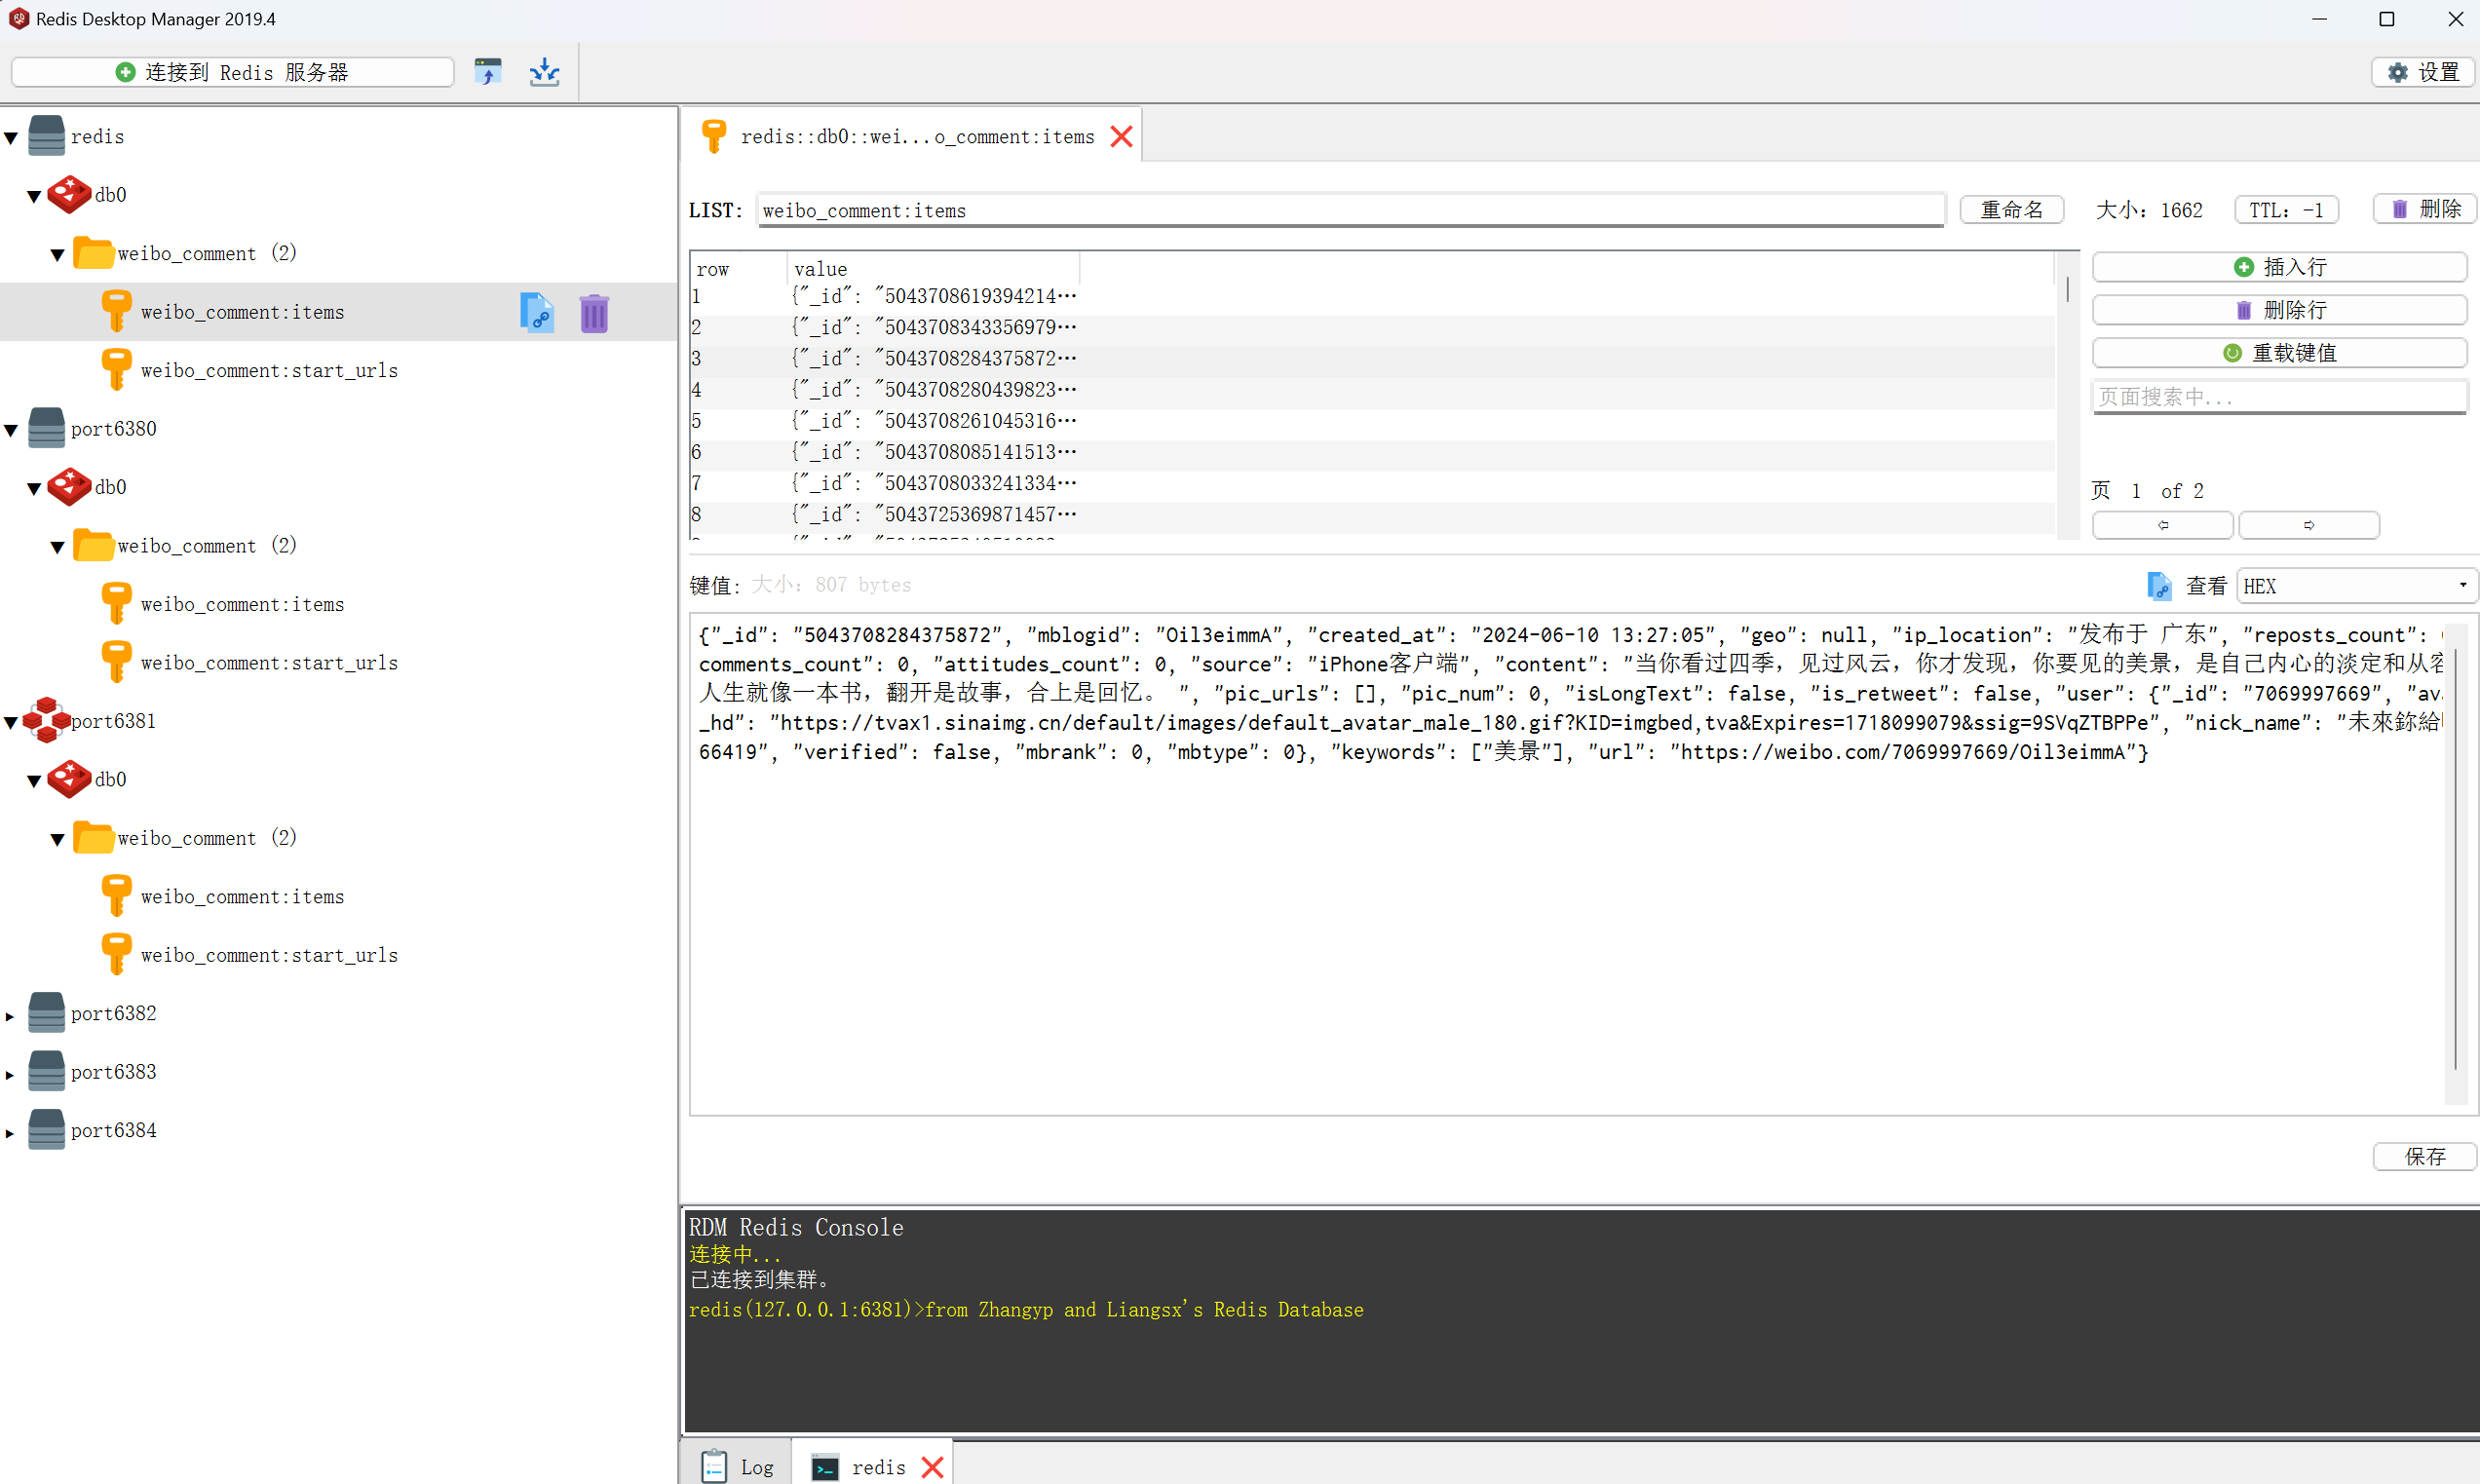
\includegraphics[width=1\textwidth]{figures/redis-manager.png}
\end{figure}


\newpage
\section{作业总结}

我们实现的项目是基于 Scrapy-Redis 的分布式爬虫系统,主要利用了 Scrapy 框架与分布式 Redis 数据库集群相结合,基于 streamlit 实现了可视化用户交互 Web 界面,旨在为大型、分布式的网络爬虫提供支持以及设计一个对微博推文的排名管理系统。

\begin{itemize}
    \item \texttt{实现 Scrapy 爬虫}
\end{itemize}

我们实现了一个基于 Scrapy 的爬虫,通过关键词搜索微博推文数据。通过使用 Redis 进行任务调度,利用集群存储爬取的 URL,支持按照设定的时间段和关键词进行搜索。程序通过解析响应页面,提取微博推文的相关信息,包括推文内容、发布时间、地理位置、转发数、评论数、点赞数等,支持对长微博进行完整内容的抓取。在 Pipeline 中,我们定义了两个 Scrapy Pipeline 类,用于处理爬虫爬取到的数据,爬取的数据可以写入到分布式集群中,也可以直接输出到当前的 output 文件夹,可以自由选择。

\begin{itemize}
    \item \texttt{搭建 Redis 集群}
\end{itemize}

我们搭建了一个 Redis 集群,集群之中有三个Master主节点,每一个主节点都可读可写,节点之间会互相通信,两两相连,无中心节点。在Redis-Cluster集群中,我们给每一个主节点添加从节点,主节点和从节点直接遵循主从复制模型的特性。所以最后是一个三主三从的集群模式,端口号为6379、6380、6381的为主节点,6382、6383、6384分别是对应上述几个主节点的从节点。

此外,在排名任务中,我们使用了远程过程调用。使用 Redis 作为消息代理,基于分布式缓存和消息队列的方法,来对数据库数据进行排名计算,考虑使用 Redis 的 zset 数据结构来实现排名计算,因为它天然地支持排序和排名功能。通过消息队列,我们可以将任务异步地发送到不同的节点进行处理,从而实现并行处理和任务分发。

\begin{itemize}
    \item \texttt{简单实现排名可视化}
\end{itemize}

最后我们利用 Streamlit 构建了一个简单的 Web 应用程序,用于连接和查询 Redis 数据库中的数据。我们实现了分布式排名计算,在交互界面会选择一个端口号的 Redis 作为命令的发布者,发布者将需要排序的数据信息作为消息发布到消息队列中。每个处理节点从消息队列中获取数据,并进行排序,最后归并到一个节点上进行输出。

\section{分工情况}

张宇鹏同学主要负责爬虫框架搭建,提出 Scrapy-Redis 分布式设想,搭建了一主二从复制架构,负责 Streamlit 可视化及分布式搜索的代码编写,还有主要负责 Latex 的报告、README.md文档、项目路线的撰写;梁帅轩同学主要负责 Redis-cluster 的搭建,实现了三主三从以及数据采集,数据分析,报告撰写的部分。

\end{document}
